\chapter{Specific Requirements}

\section{External Interface Requirements}

\subsection{User Interfaces}

In this section we describe and present a possible mock-up for the application, following the order of events proposed in the sequence diagrams.\\

At the launch of the application the user has to insert the credentials in the Log In page~\ref{fig:LogInMockup}. In case of new user, he can click on a button to open the Sign Up page~\ref{fig:SignUpMockup}, to create a new account.

% screenshots here
\begin{figure}[H]
	\centering     %%% not \center
	\subfigure[Log In page.]{\label{fig:LogInMockup}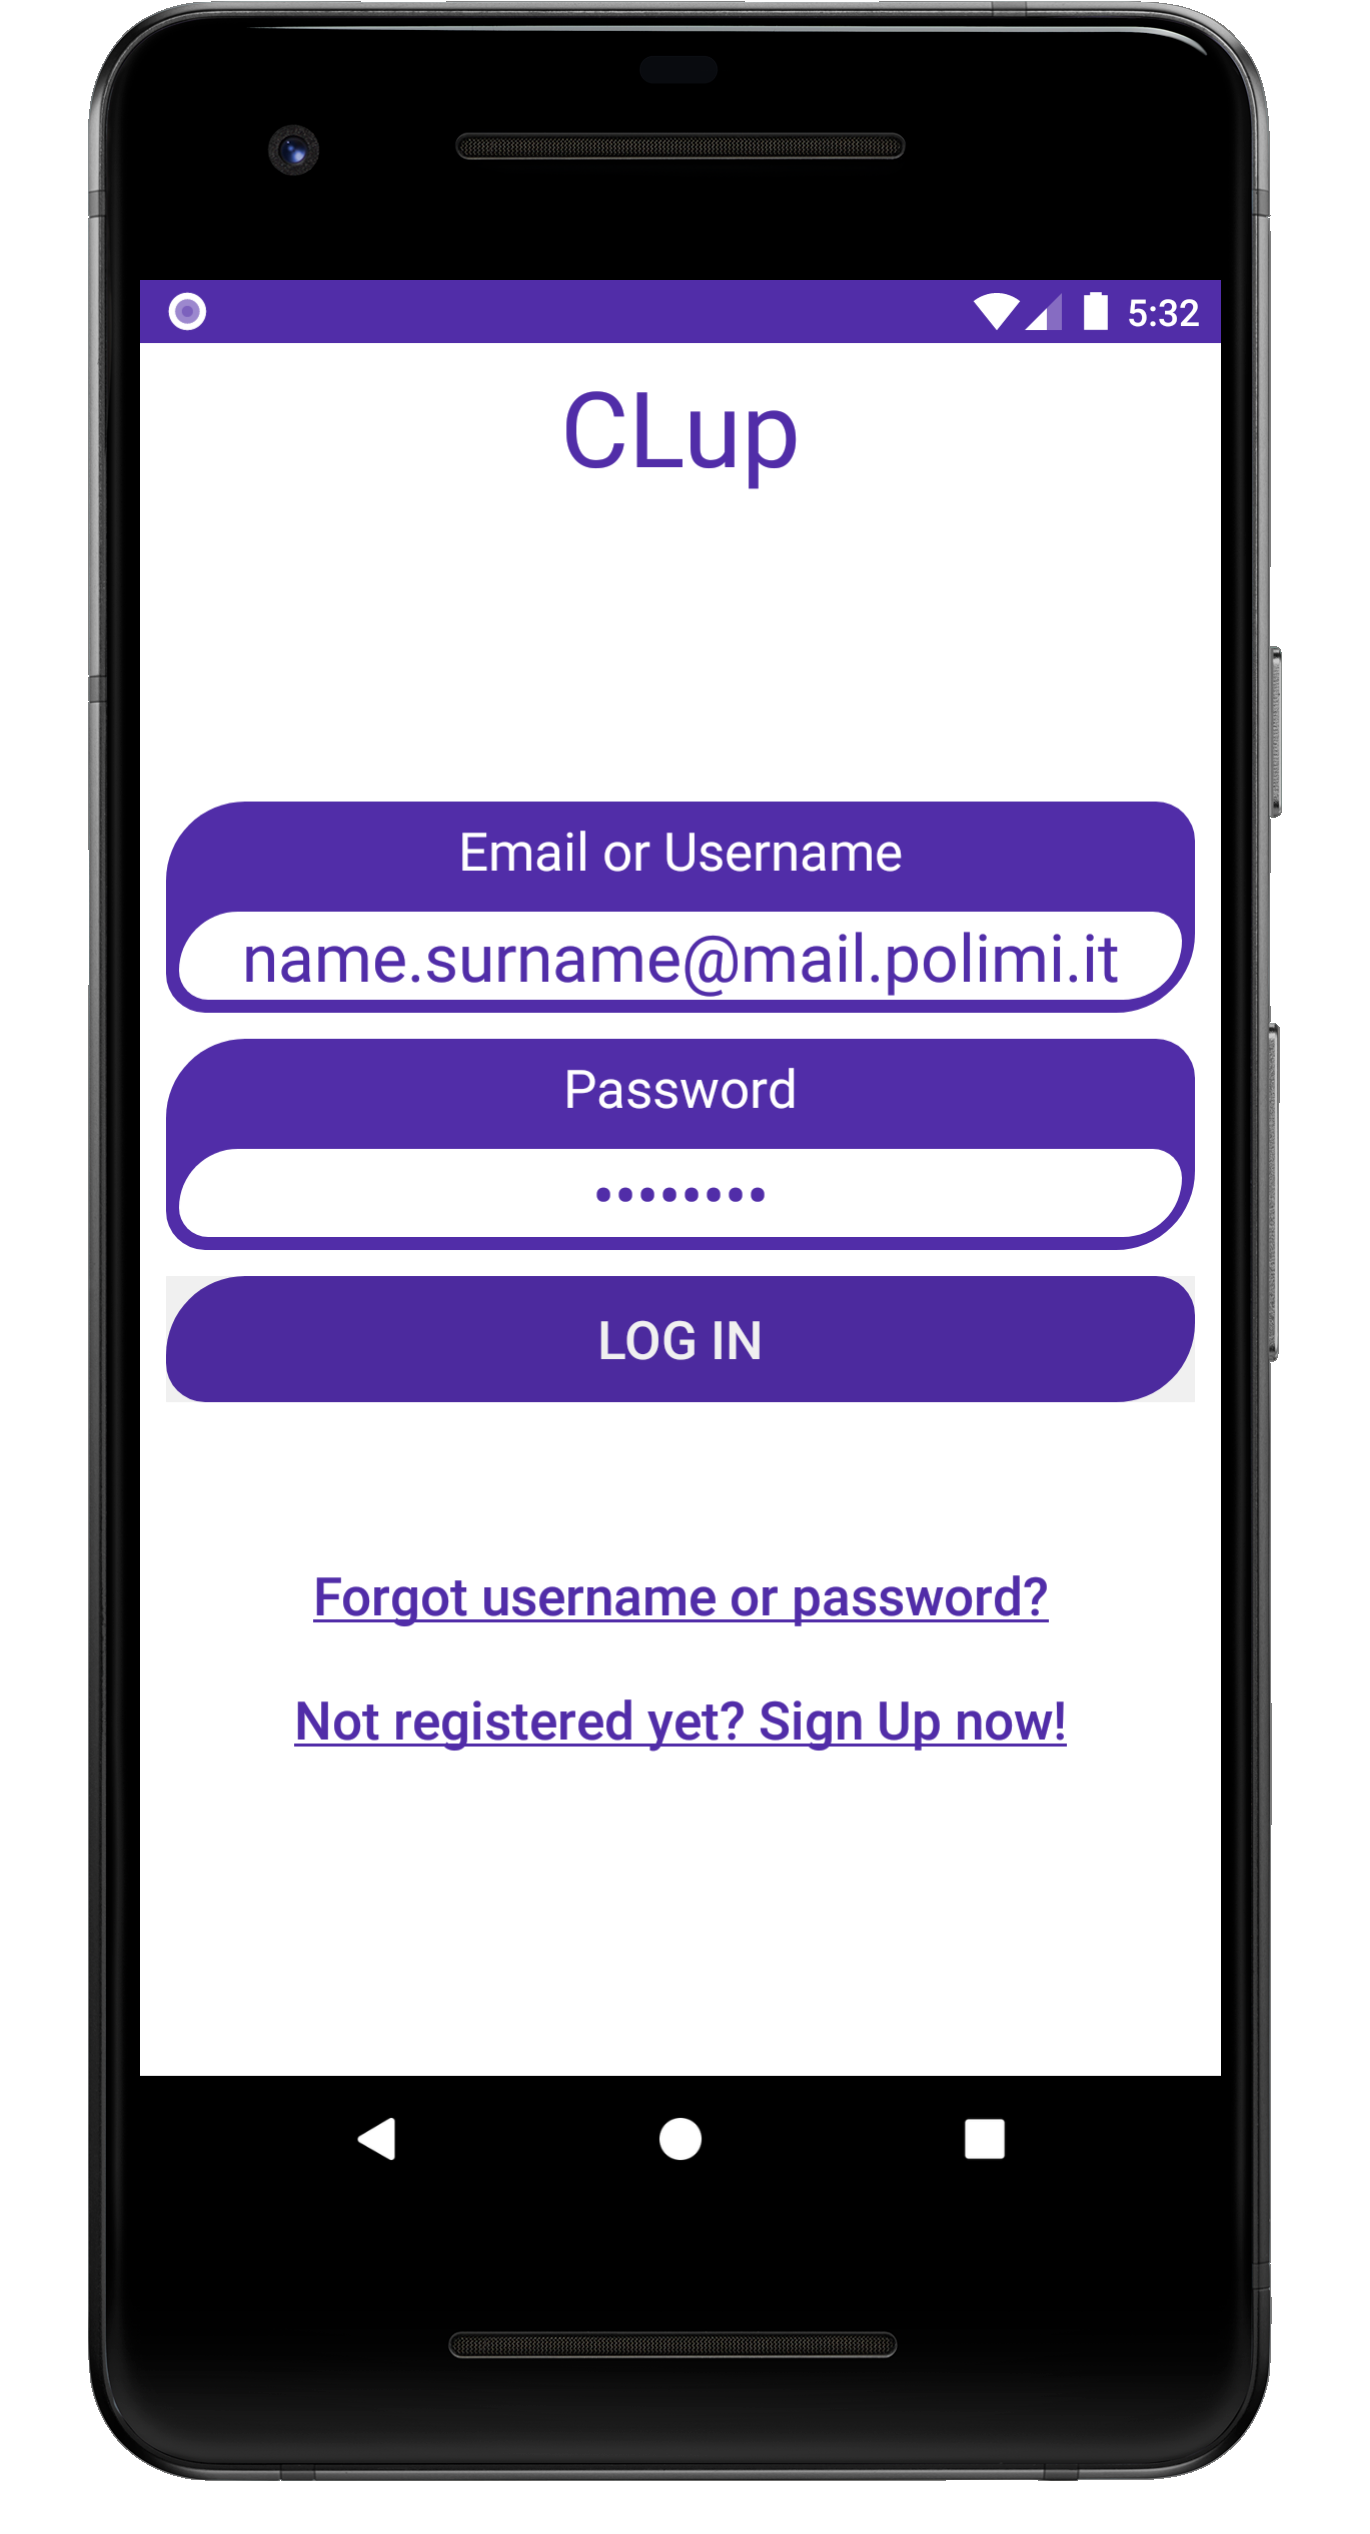
\includegraphics[width=0.3\textwidth]{images/log_in.png}}
	\subfigure[Sign Up page.]{\label{fig:SignUpMockup}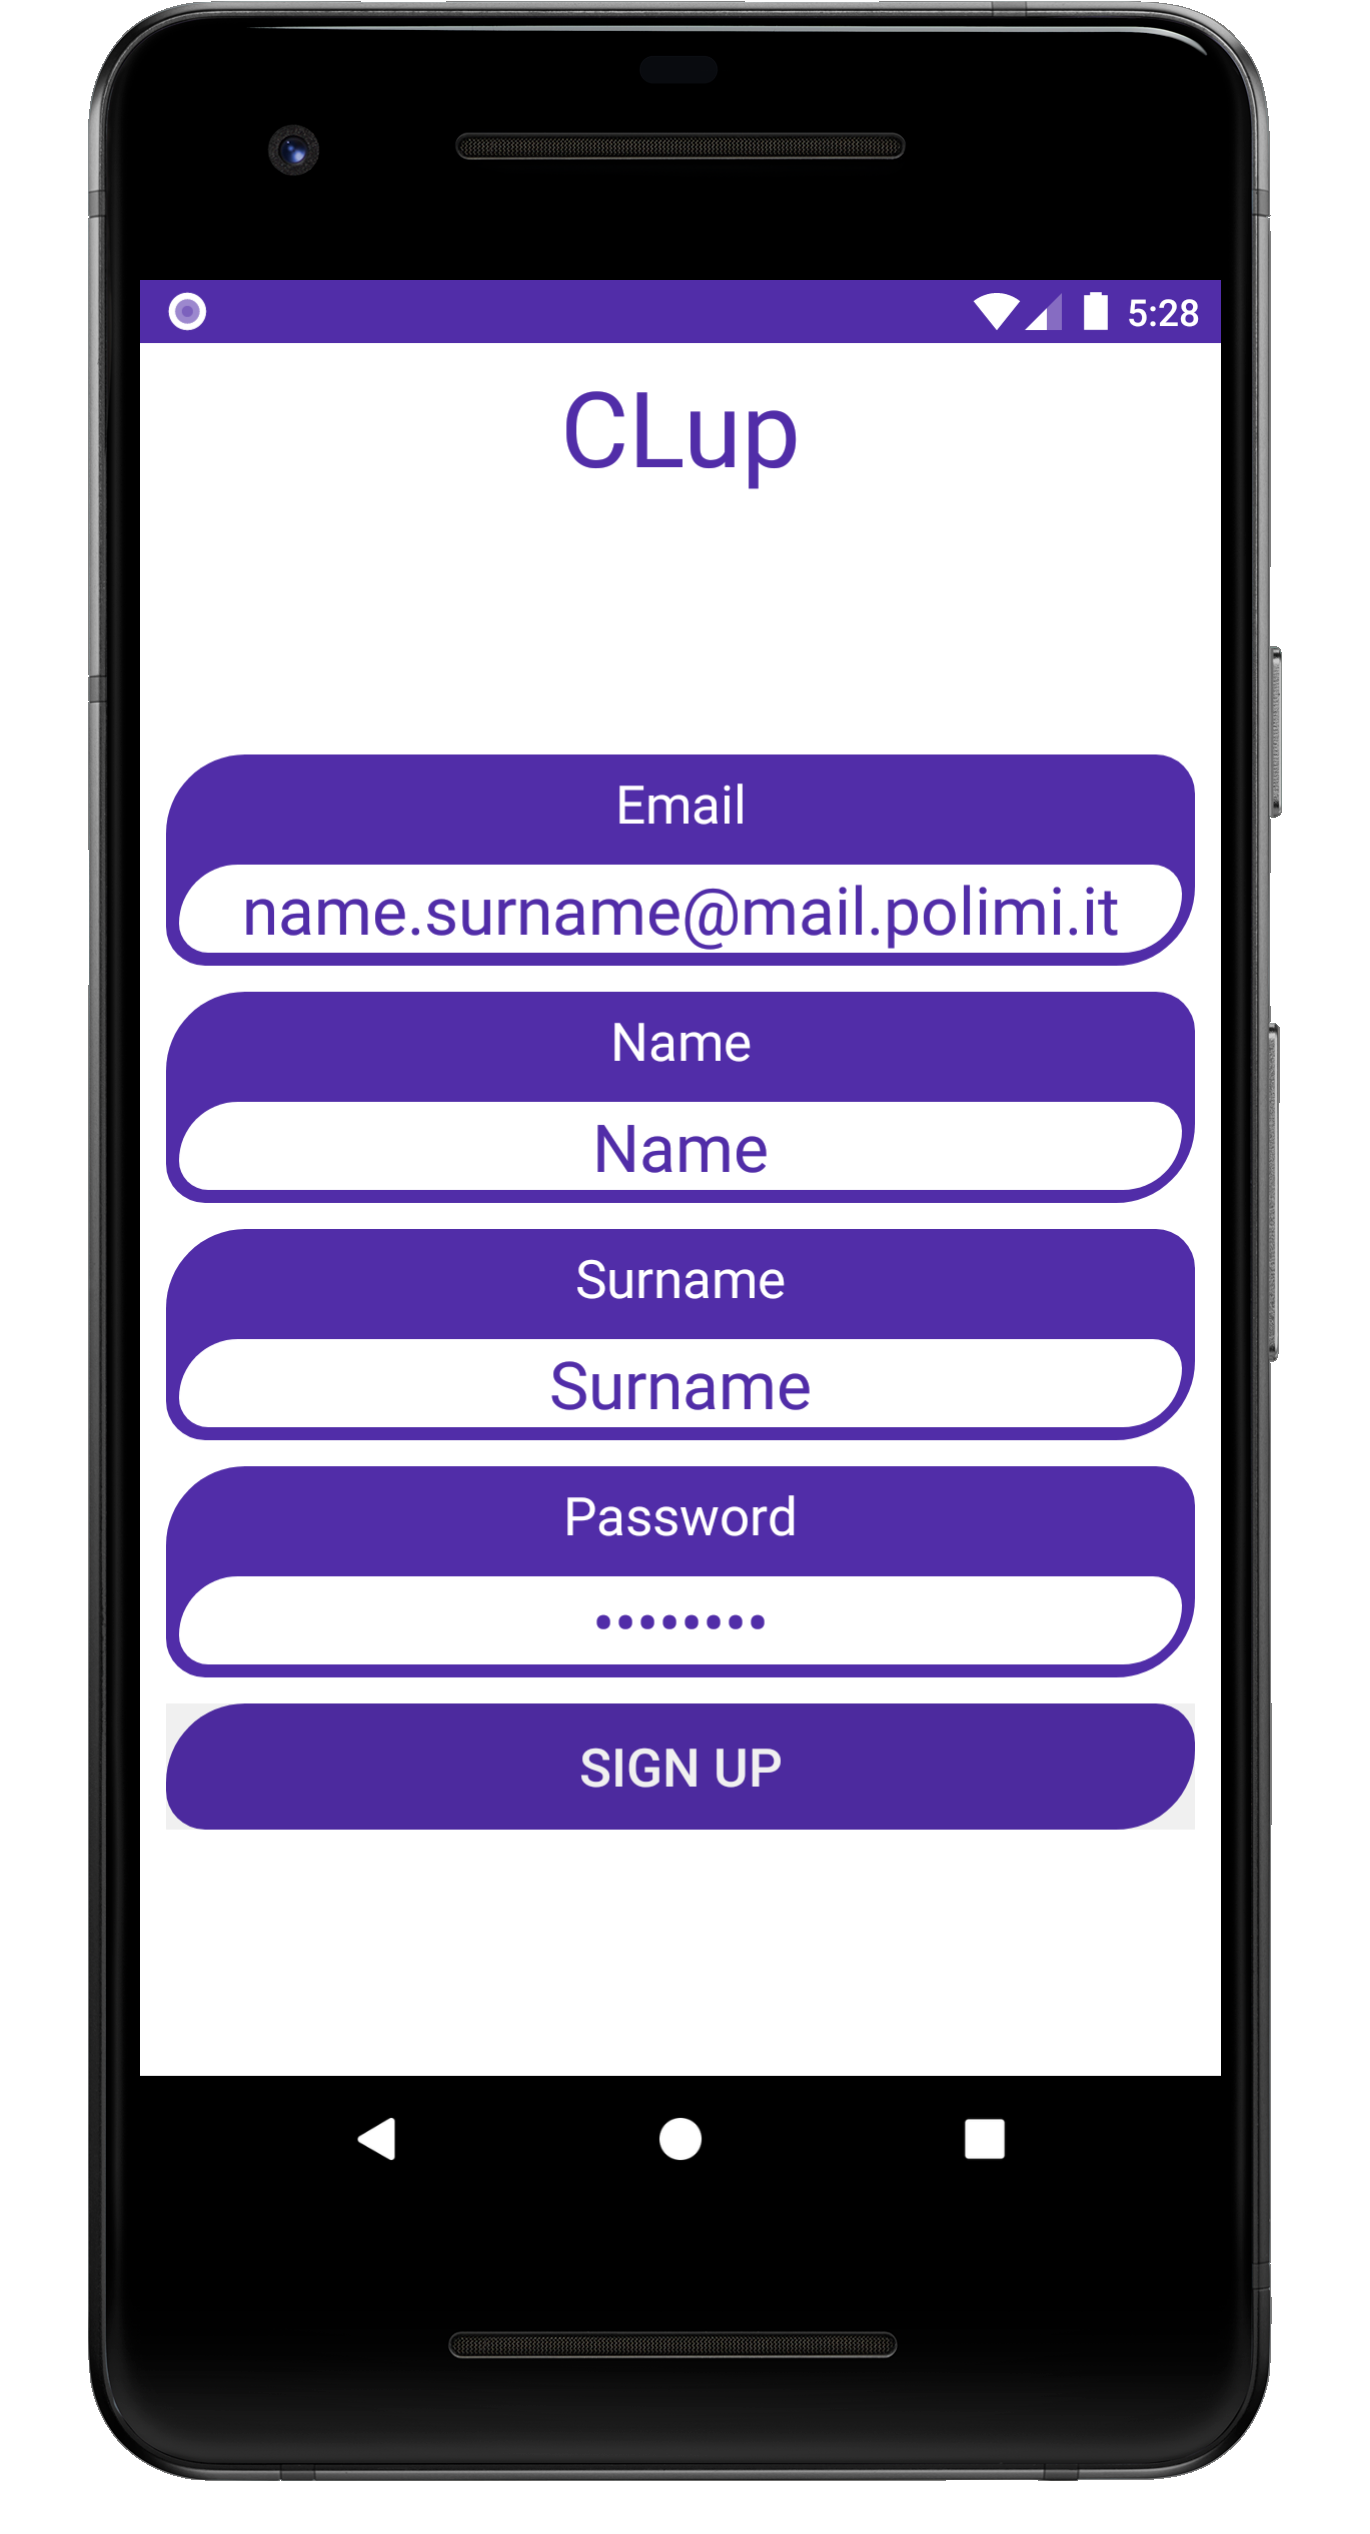
\includegraphics[width=0.3\textwidth]{images/sign_up.png}}
	\caption{Example of Log In and Sign Up pages.}
\end{figure}

Once the login has been completed successfully, the user is redirected to the Home page~\ref{fig:HomeMockup}.
In particular, the reported figure shows the Home page for the customer account with all the functionalities. The application, knowing the type of account, is able to show different buttons. For example, in case of physical spot account, the application will display only the Lining Up button, hiding the others. In case of store manager account, there will be displayed only buttons to control the queue and to analyze the statistics. 

\begin{figure}[H]
	\centering
	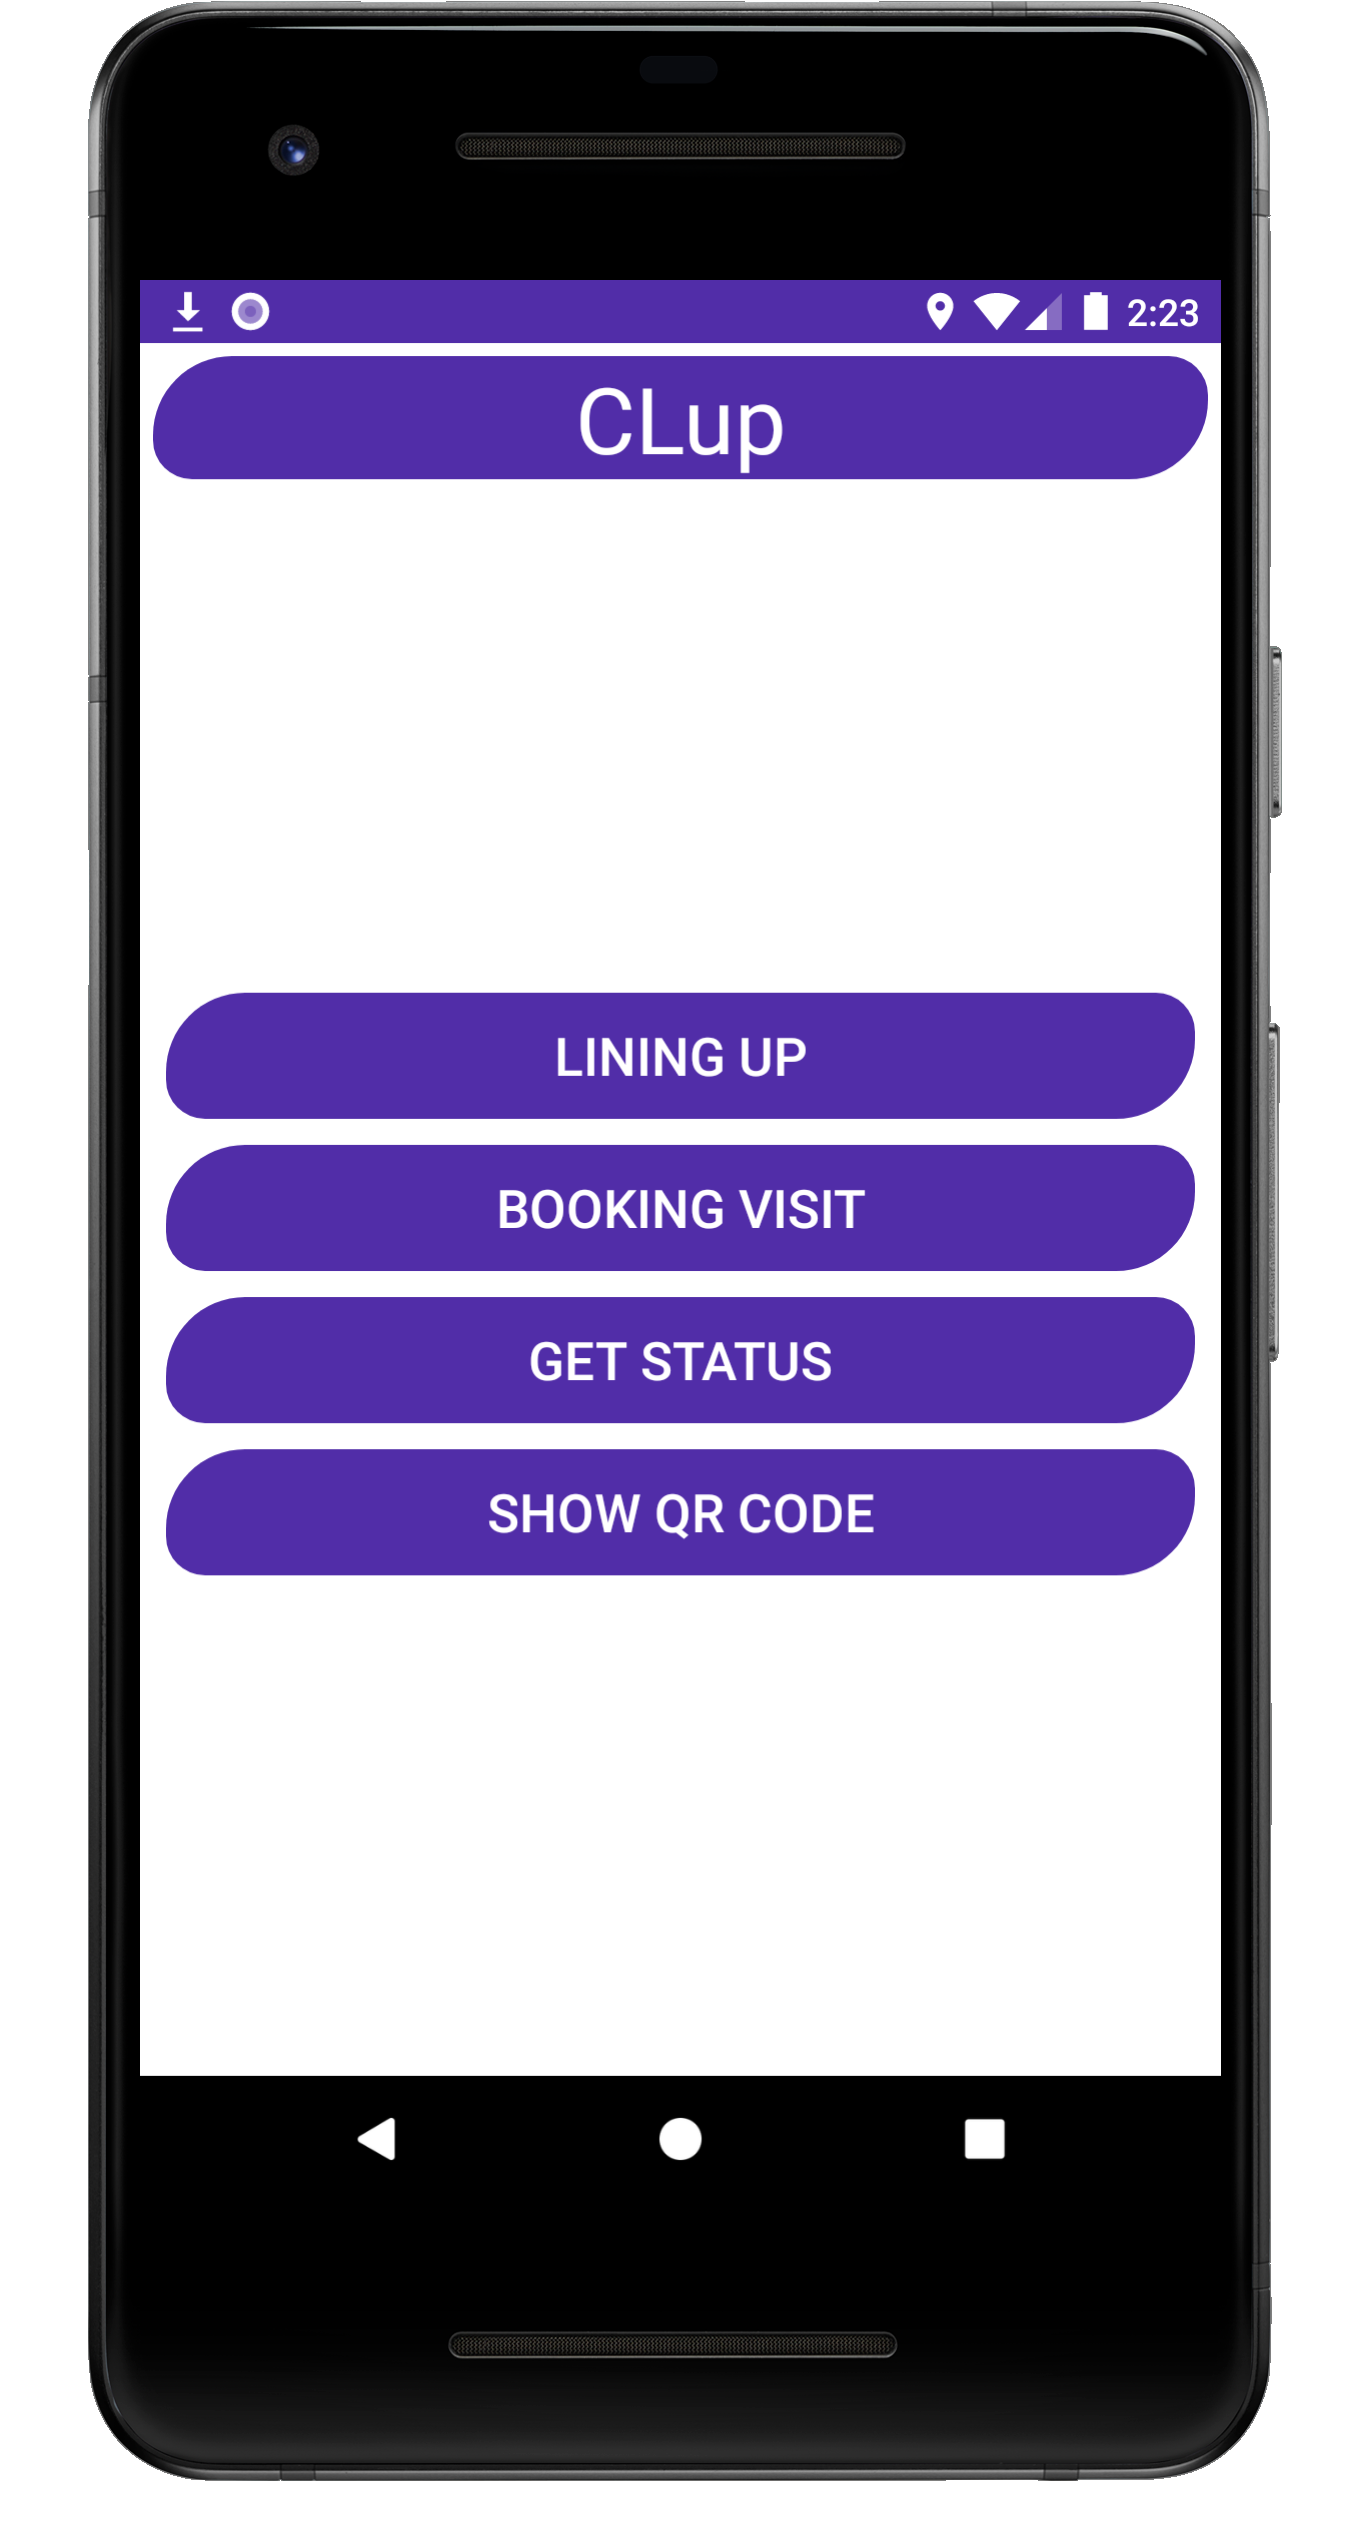
\includegraphics[width=0.3\textwidth]{images/home.png}
	\caption{Home page.}
	\label{fig:HomeMockup}
\end{figure}

If a customer wants to line up, or book a visit, he can click on the corresponding button, in this way the application will show the form to insert the requested parameters~\ref{fig:LiningBookingMockup}.
In the mock-up we show how the user can choose the store, the time slot and, in case of booking, the category of grocery, by expanding the drop down menu.

\begin{figure}[H]
	\centering     %%% not \center
	\subfigure[Lining Up page.]{\label{fig:LiningUpMockup}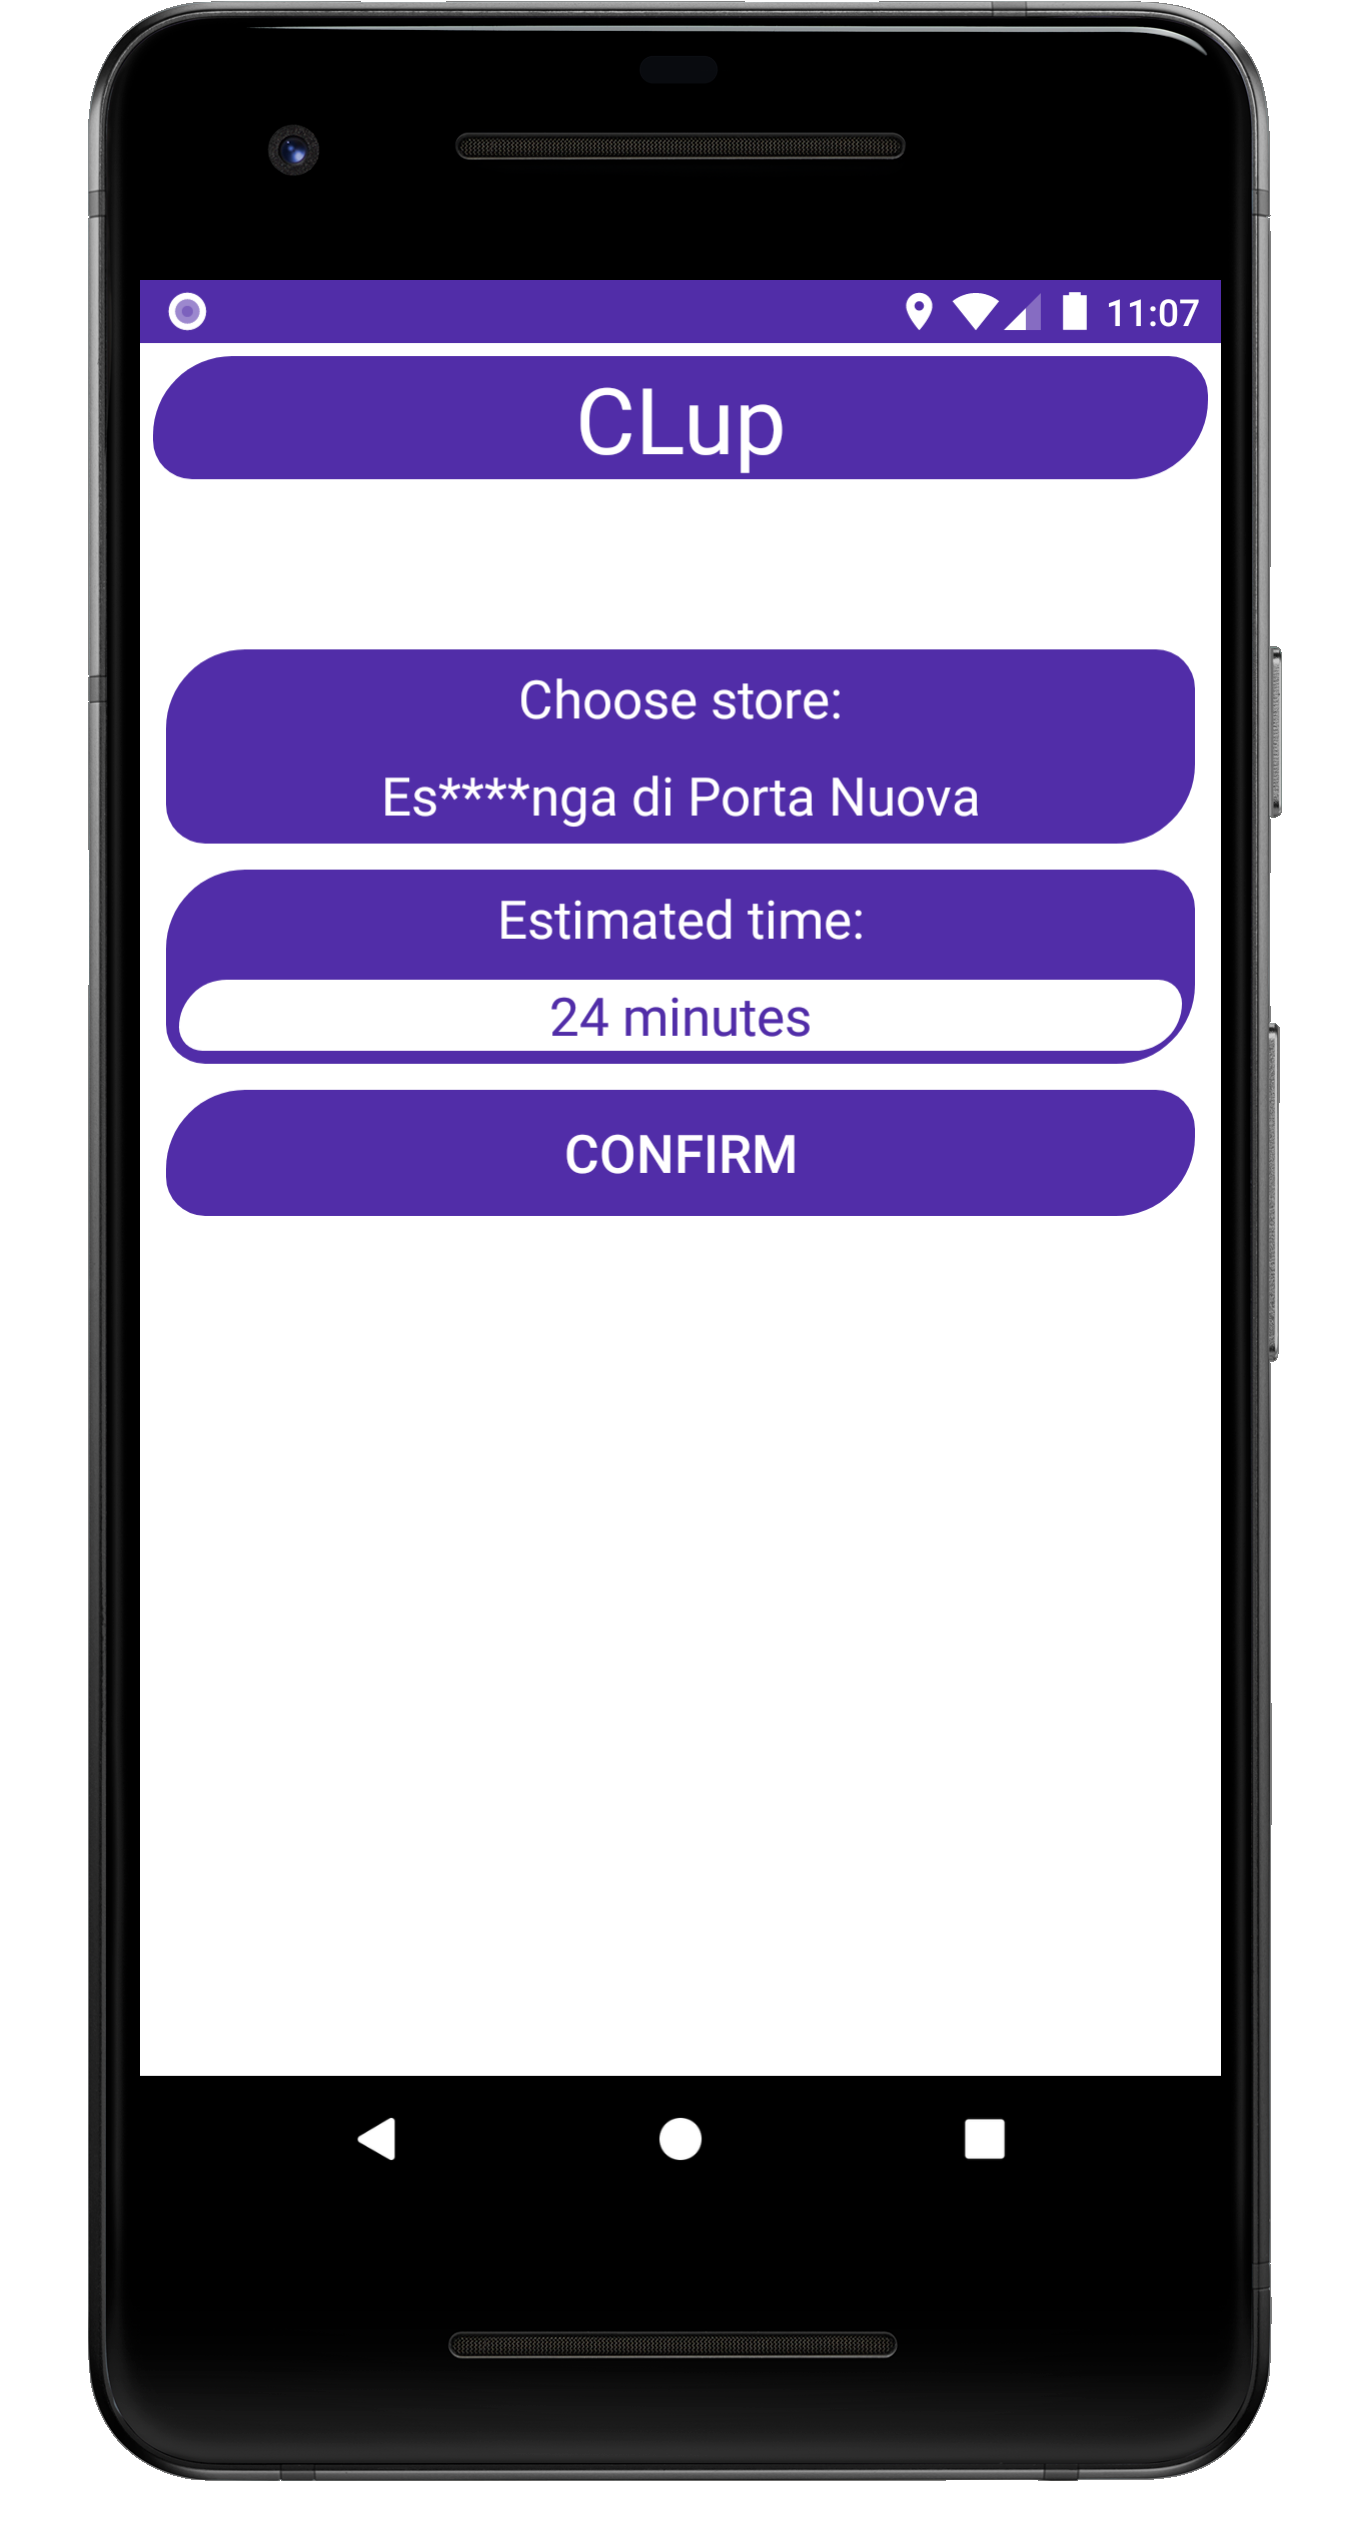
\includegraphics[width=0.3\textwidth]{images/lining_up_01.png}}
	\subfigure[Booking Visit page.]{\label{fig:BookingVisitMockup}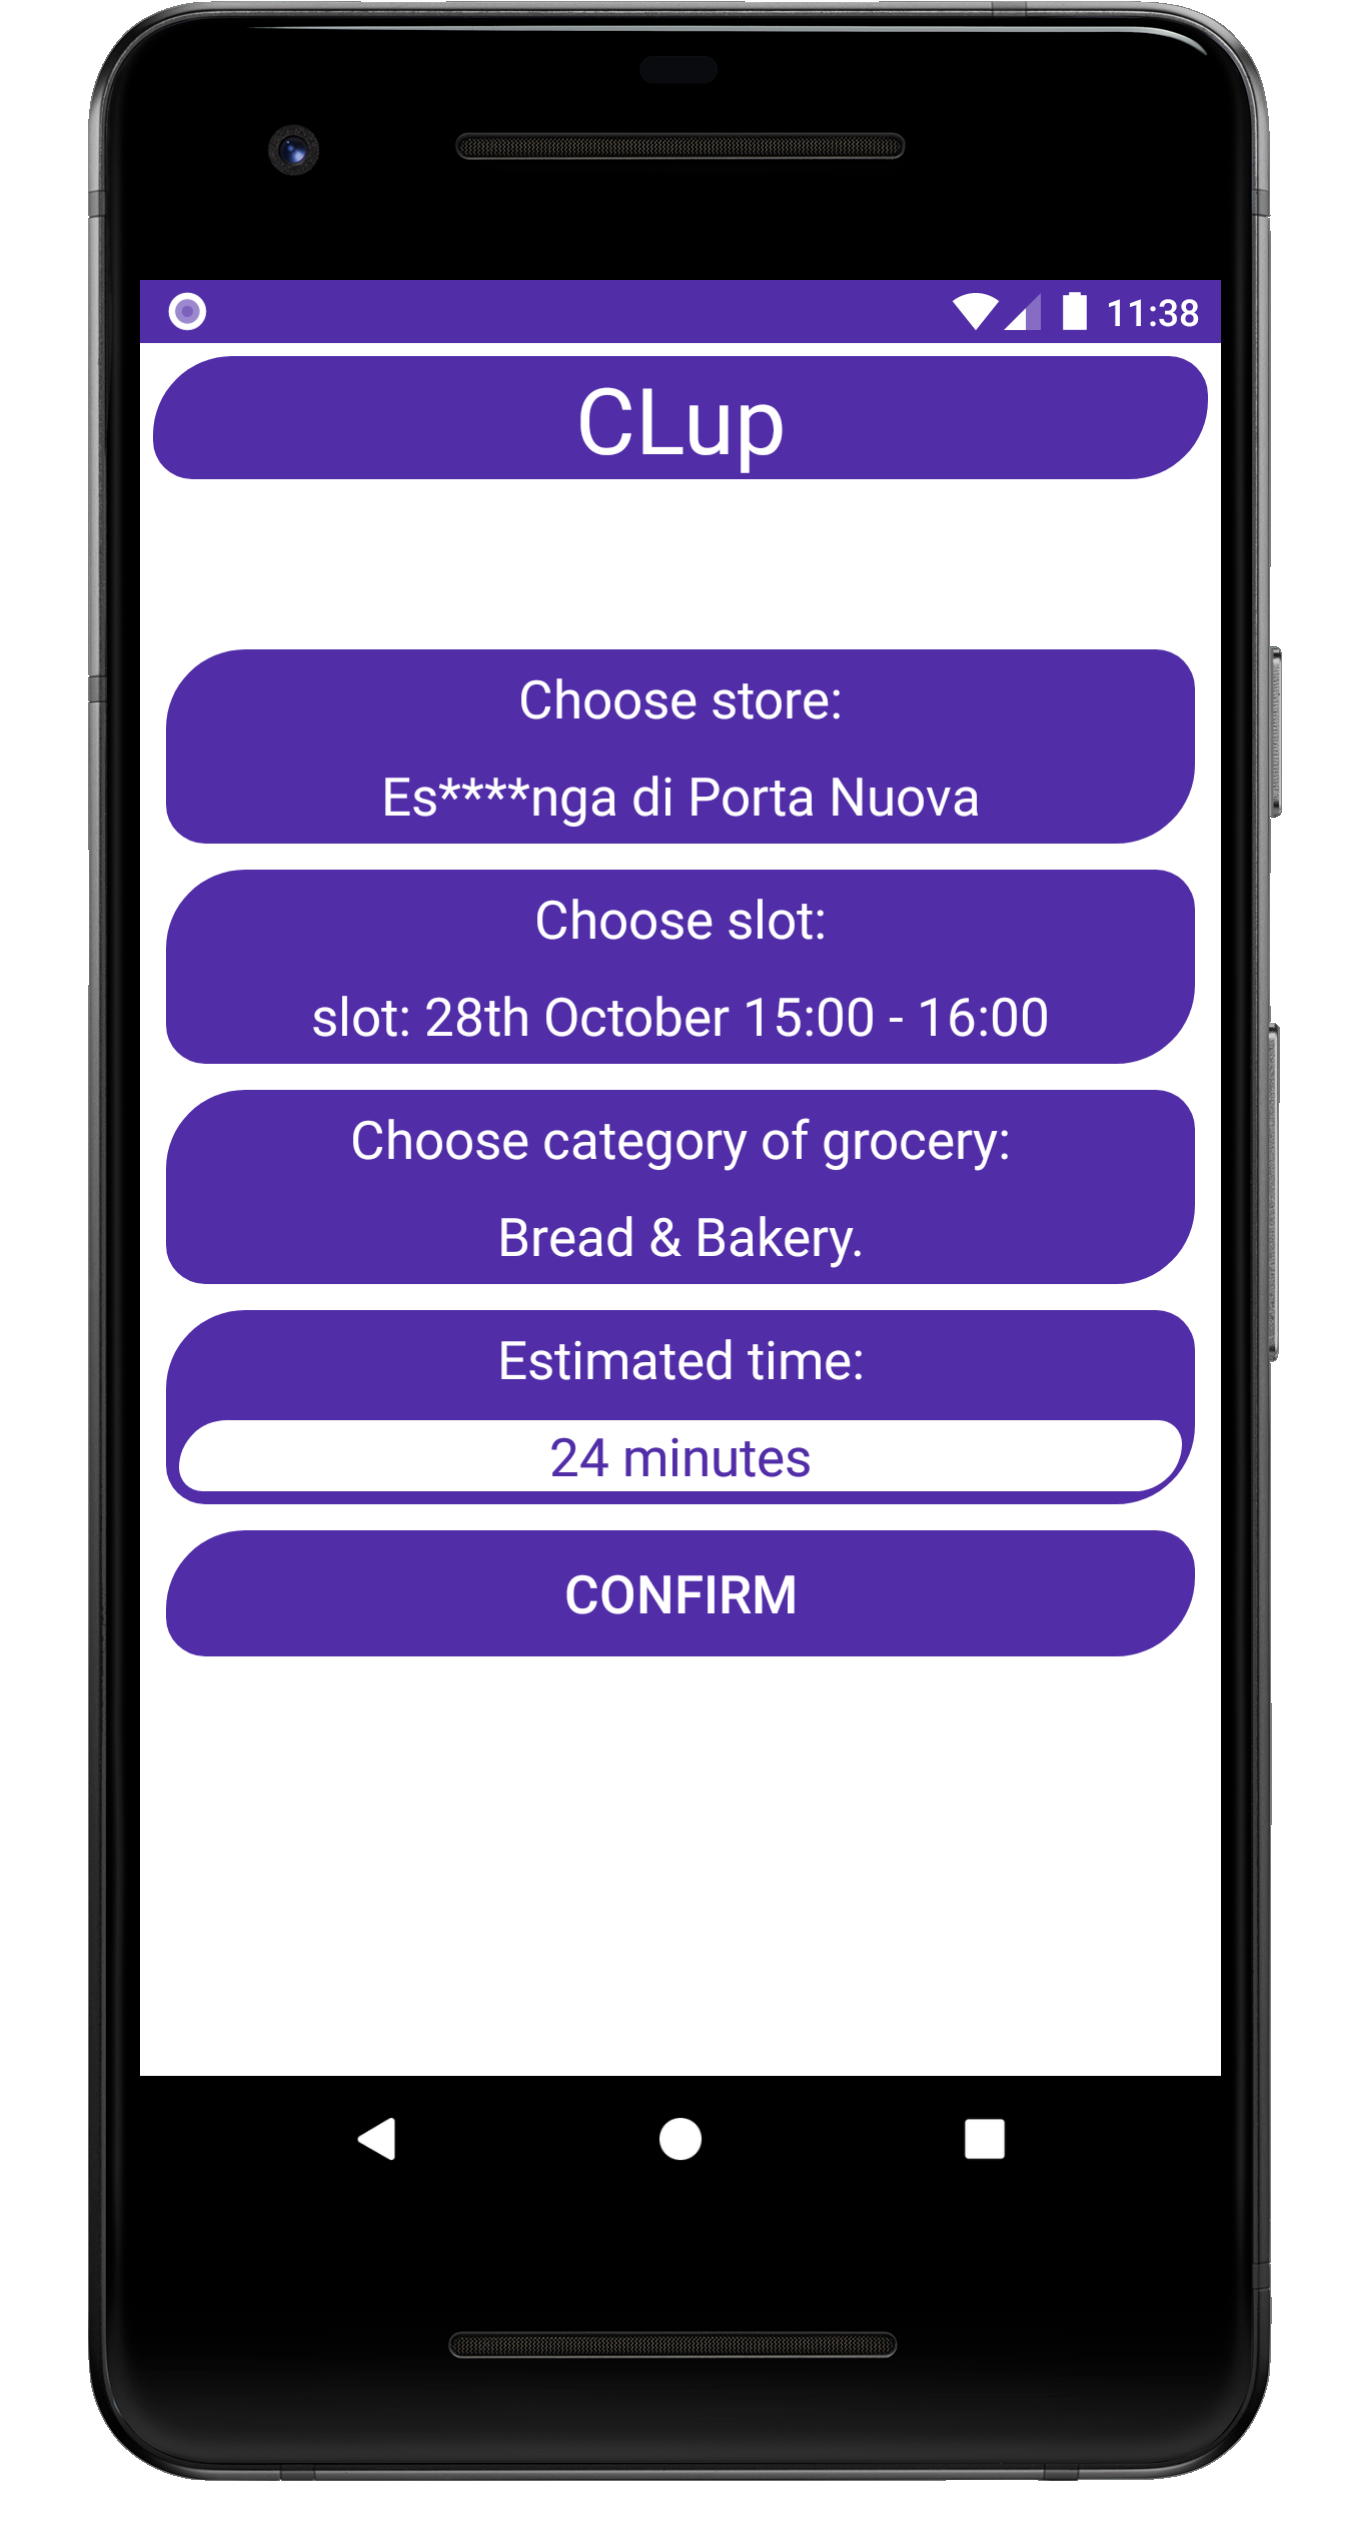
\includegraphics[width=0.3\textwidth]{images/booking_visit_01.png}}
	
	\subfigure[Lining Up page with expanded spinner.]{\label{fig:LiningUp2Mockup}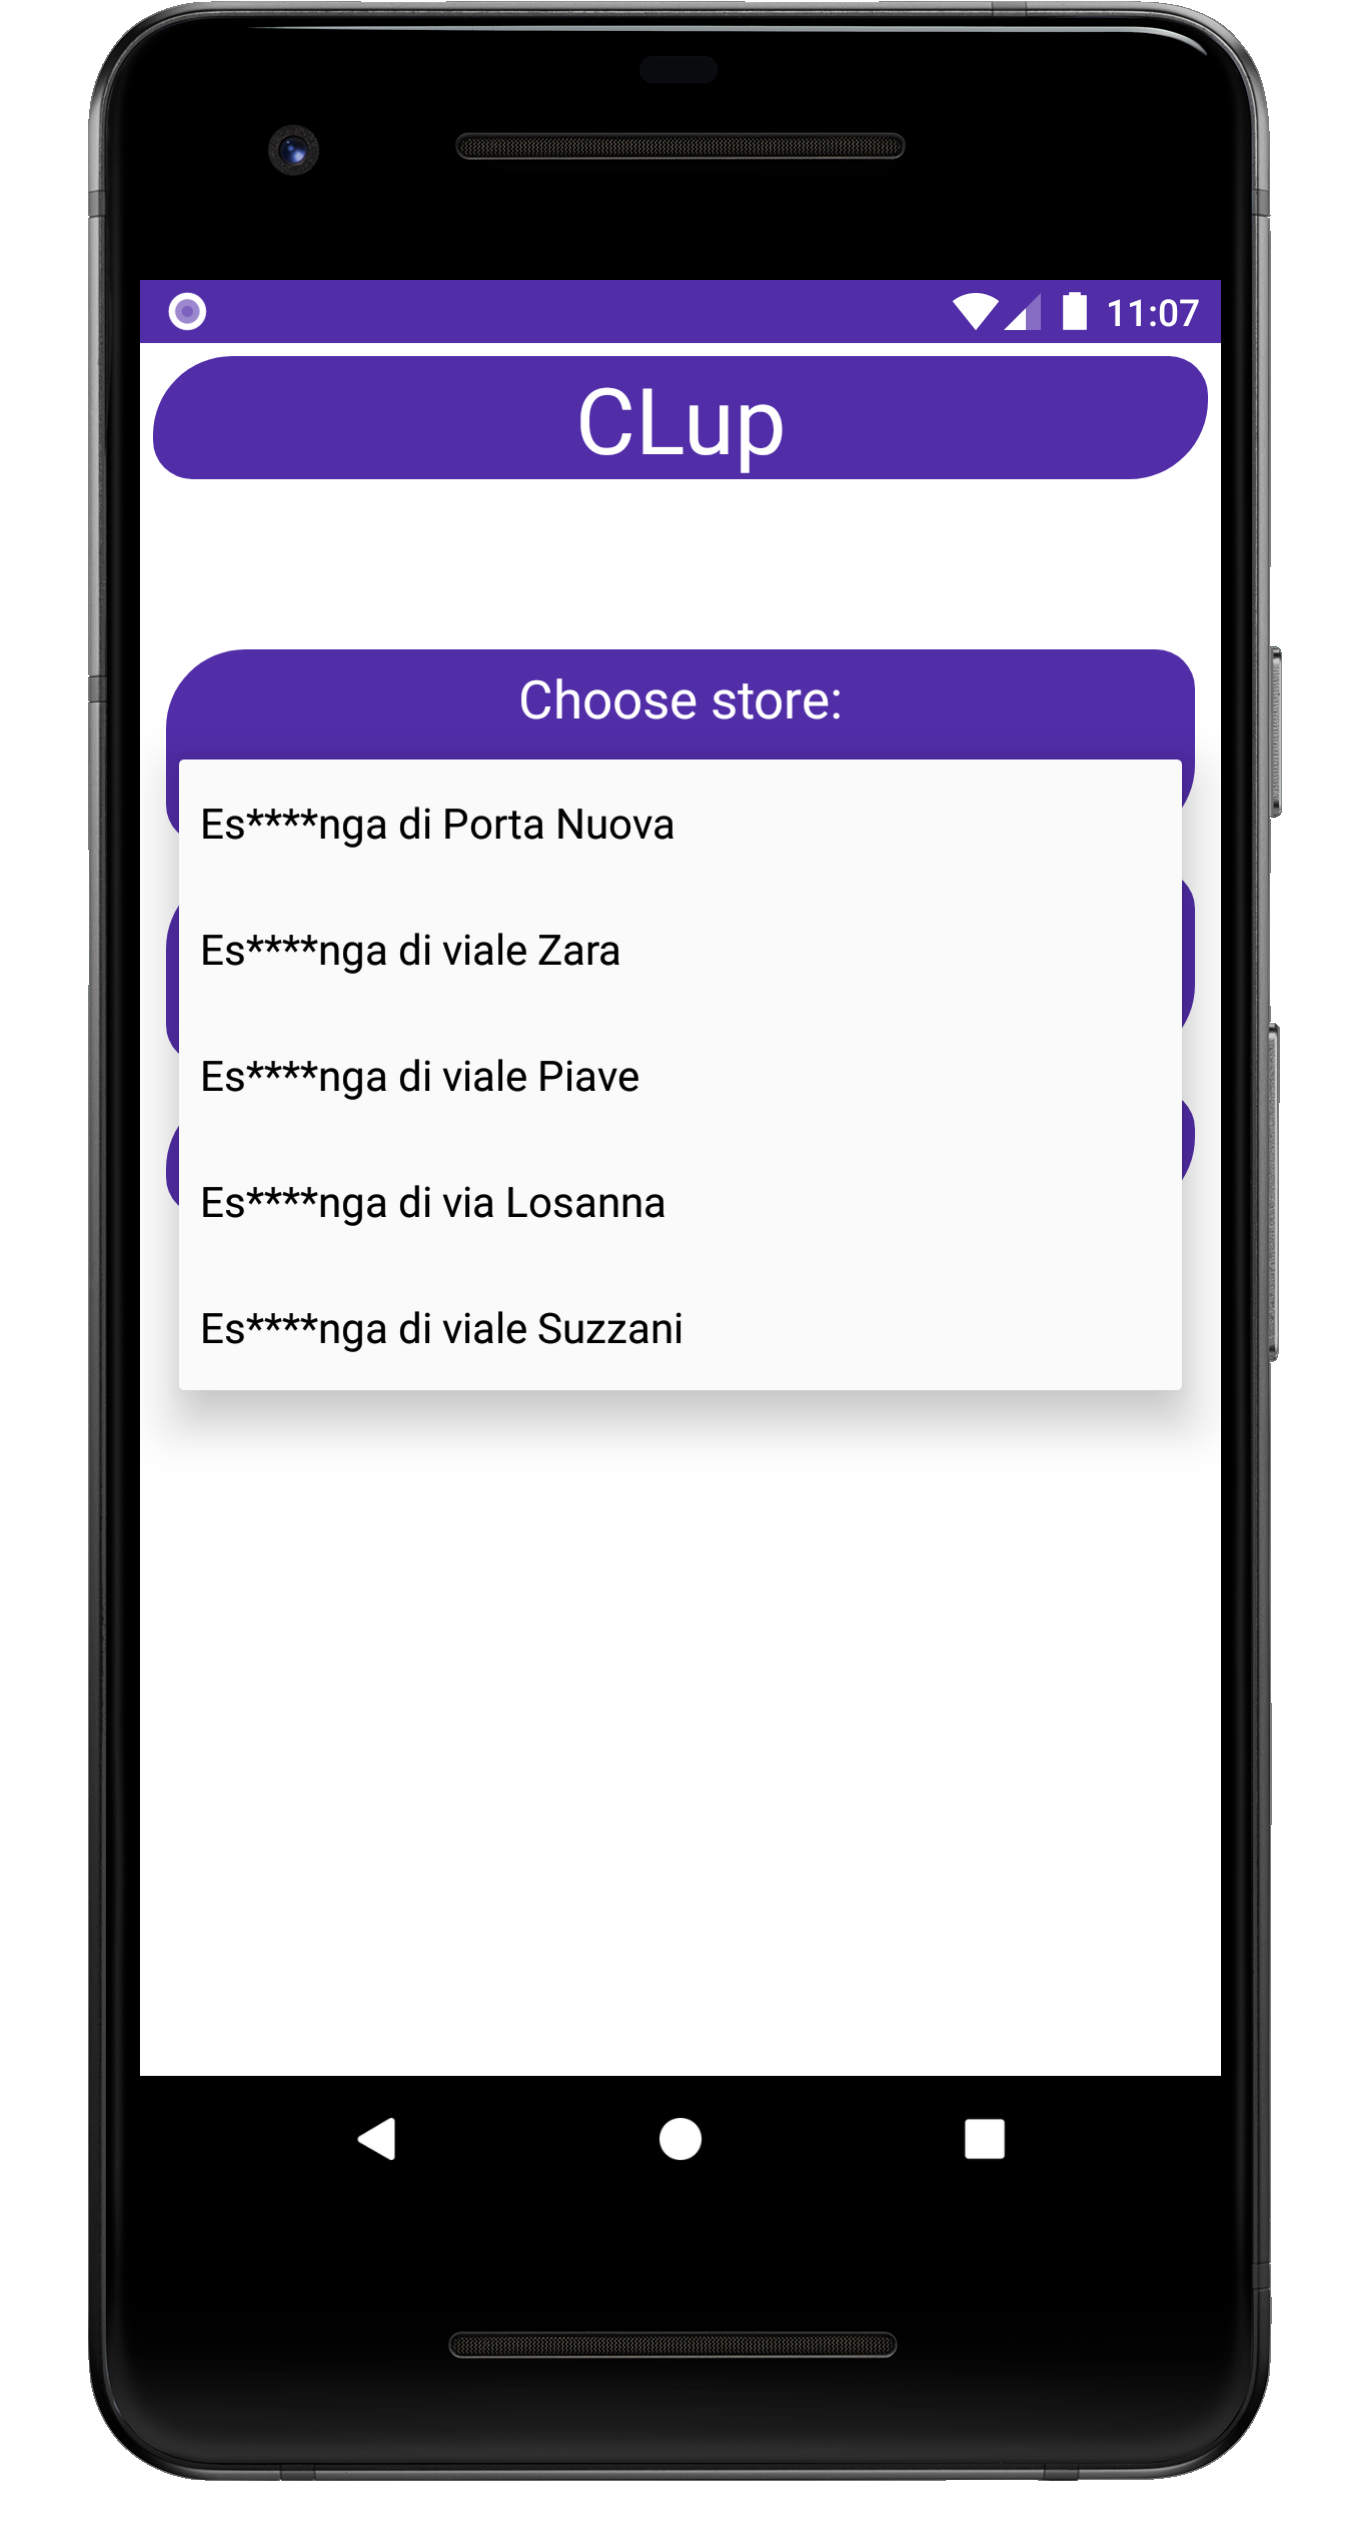
\includegraphics[width=0.3\textwidth]{images/lining_up_02.png}}
	\subfigure[Booking Visit page with expanded spinner.]{\label{fig:BookingVisit2Mockup}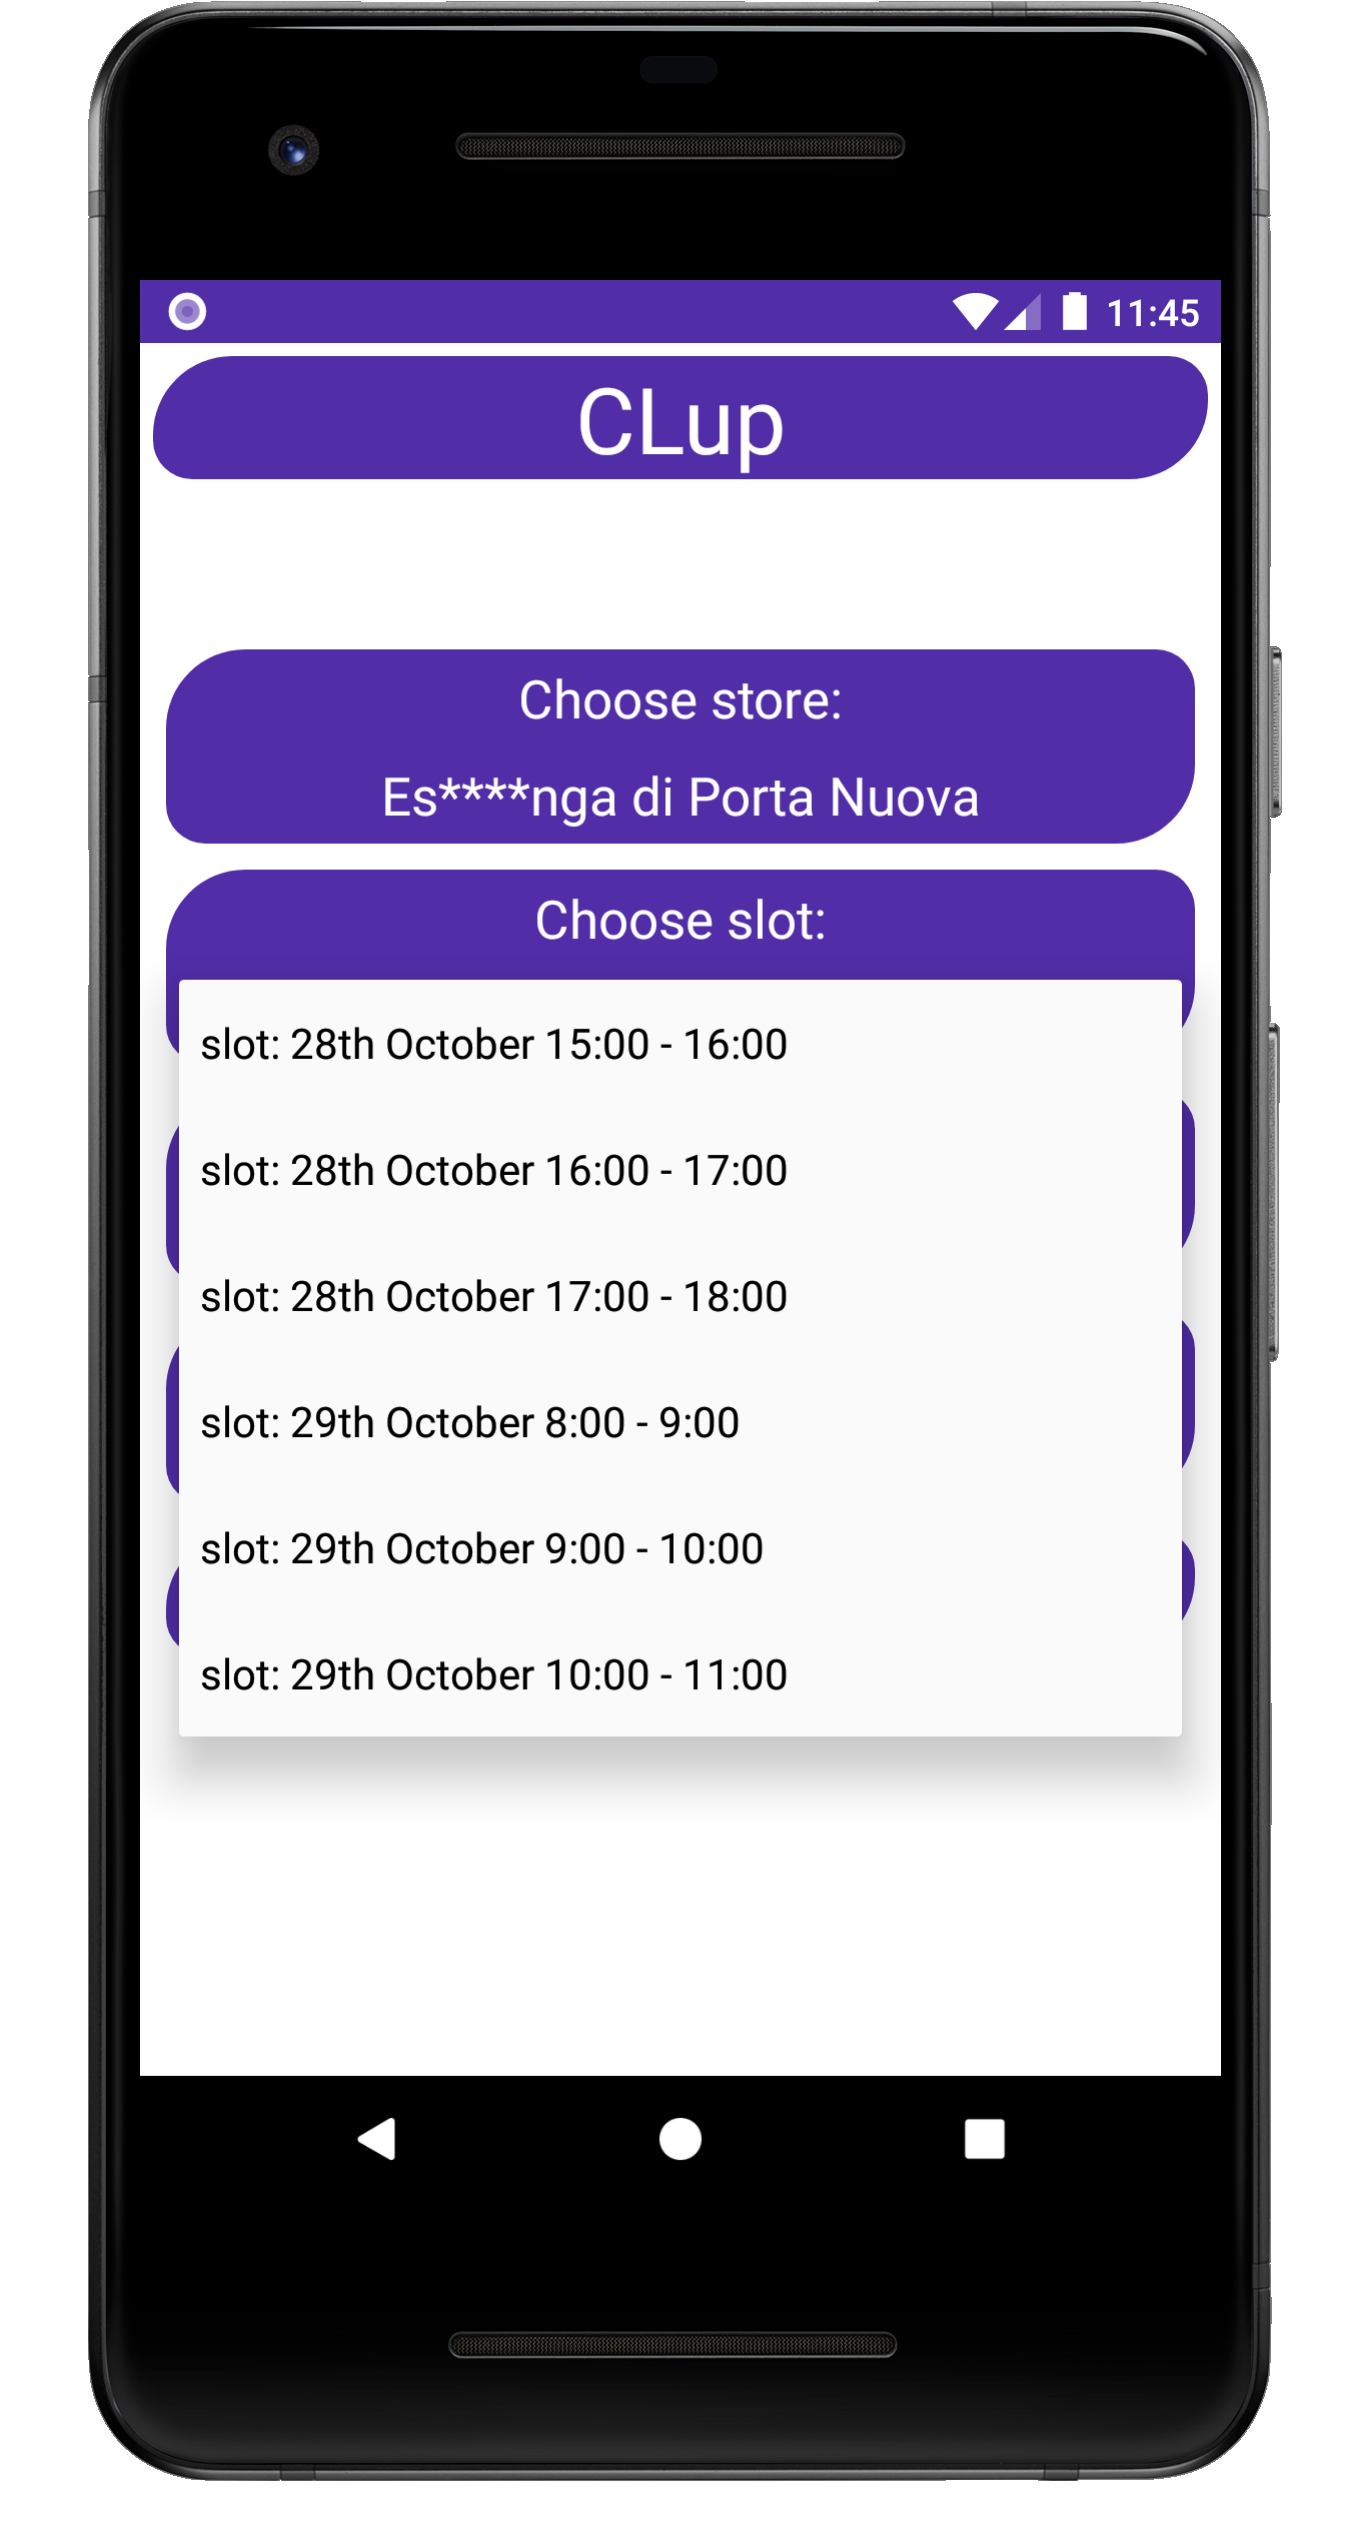
\includegraphics[width=0.3\textwidth]{images/booking_visit_02.png}}
	\caption{Example of Lining Up and Booking Visit pages.}
	\label{fig:LiningBookingMockup}
\end{figure}

The application provides the possibility to check the queue status by clicking on the Get Status button and to watch the QR code by clicking on the relative button.
These buttons aren't visible from the Home page until the user performs a lining up, or booking a visit, operation.
If visible, the users will be able to see the interfaces: \ref{fig:GetStatusMockup}, \ref{fig:ShowQRMockup}.

\begin{figure}[H]
	\centering     %%% not \center
	\subfigure[Status page.]{\label{fig:GetStatusMockup}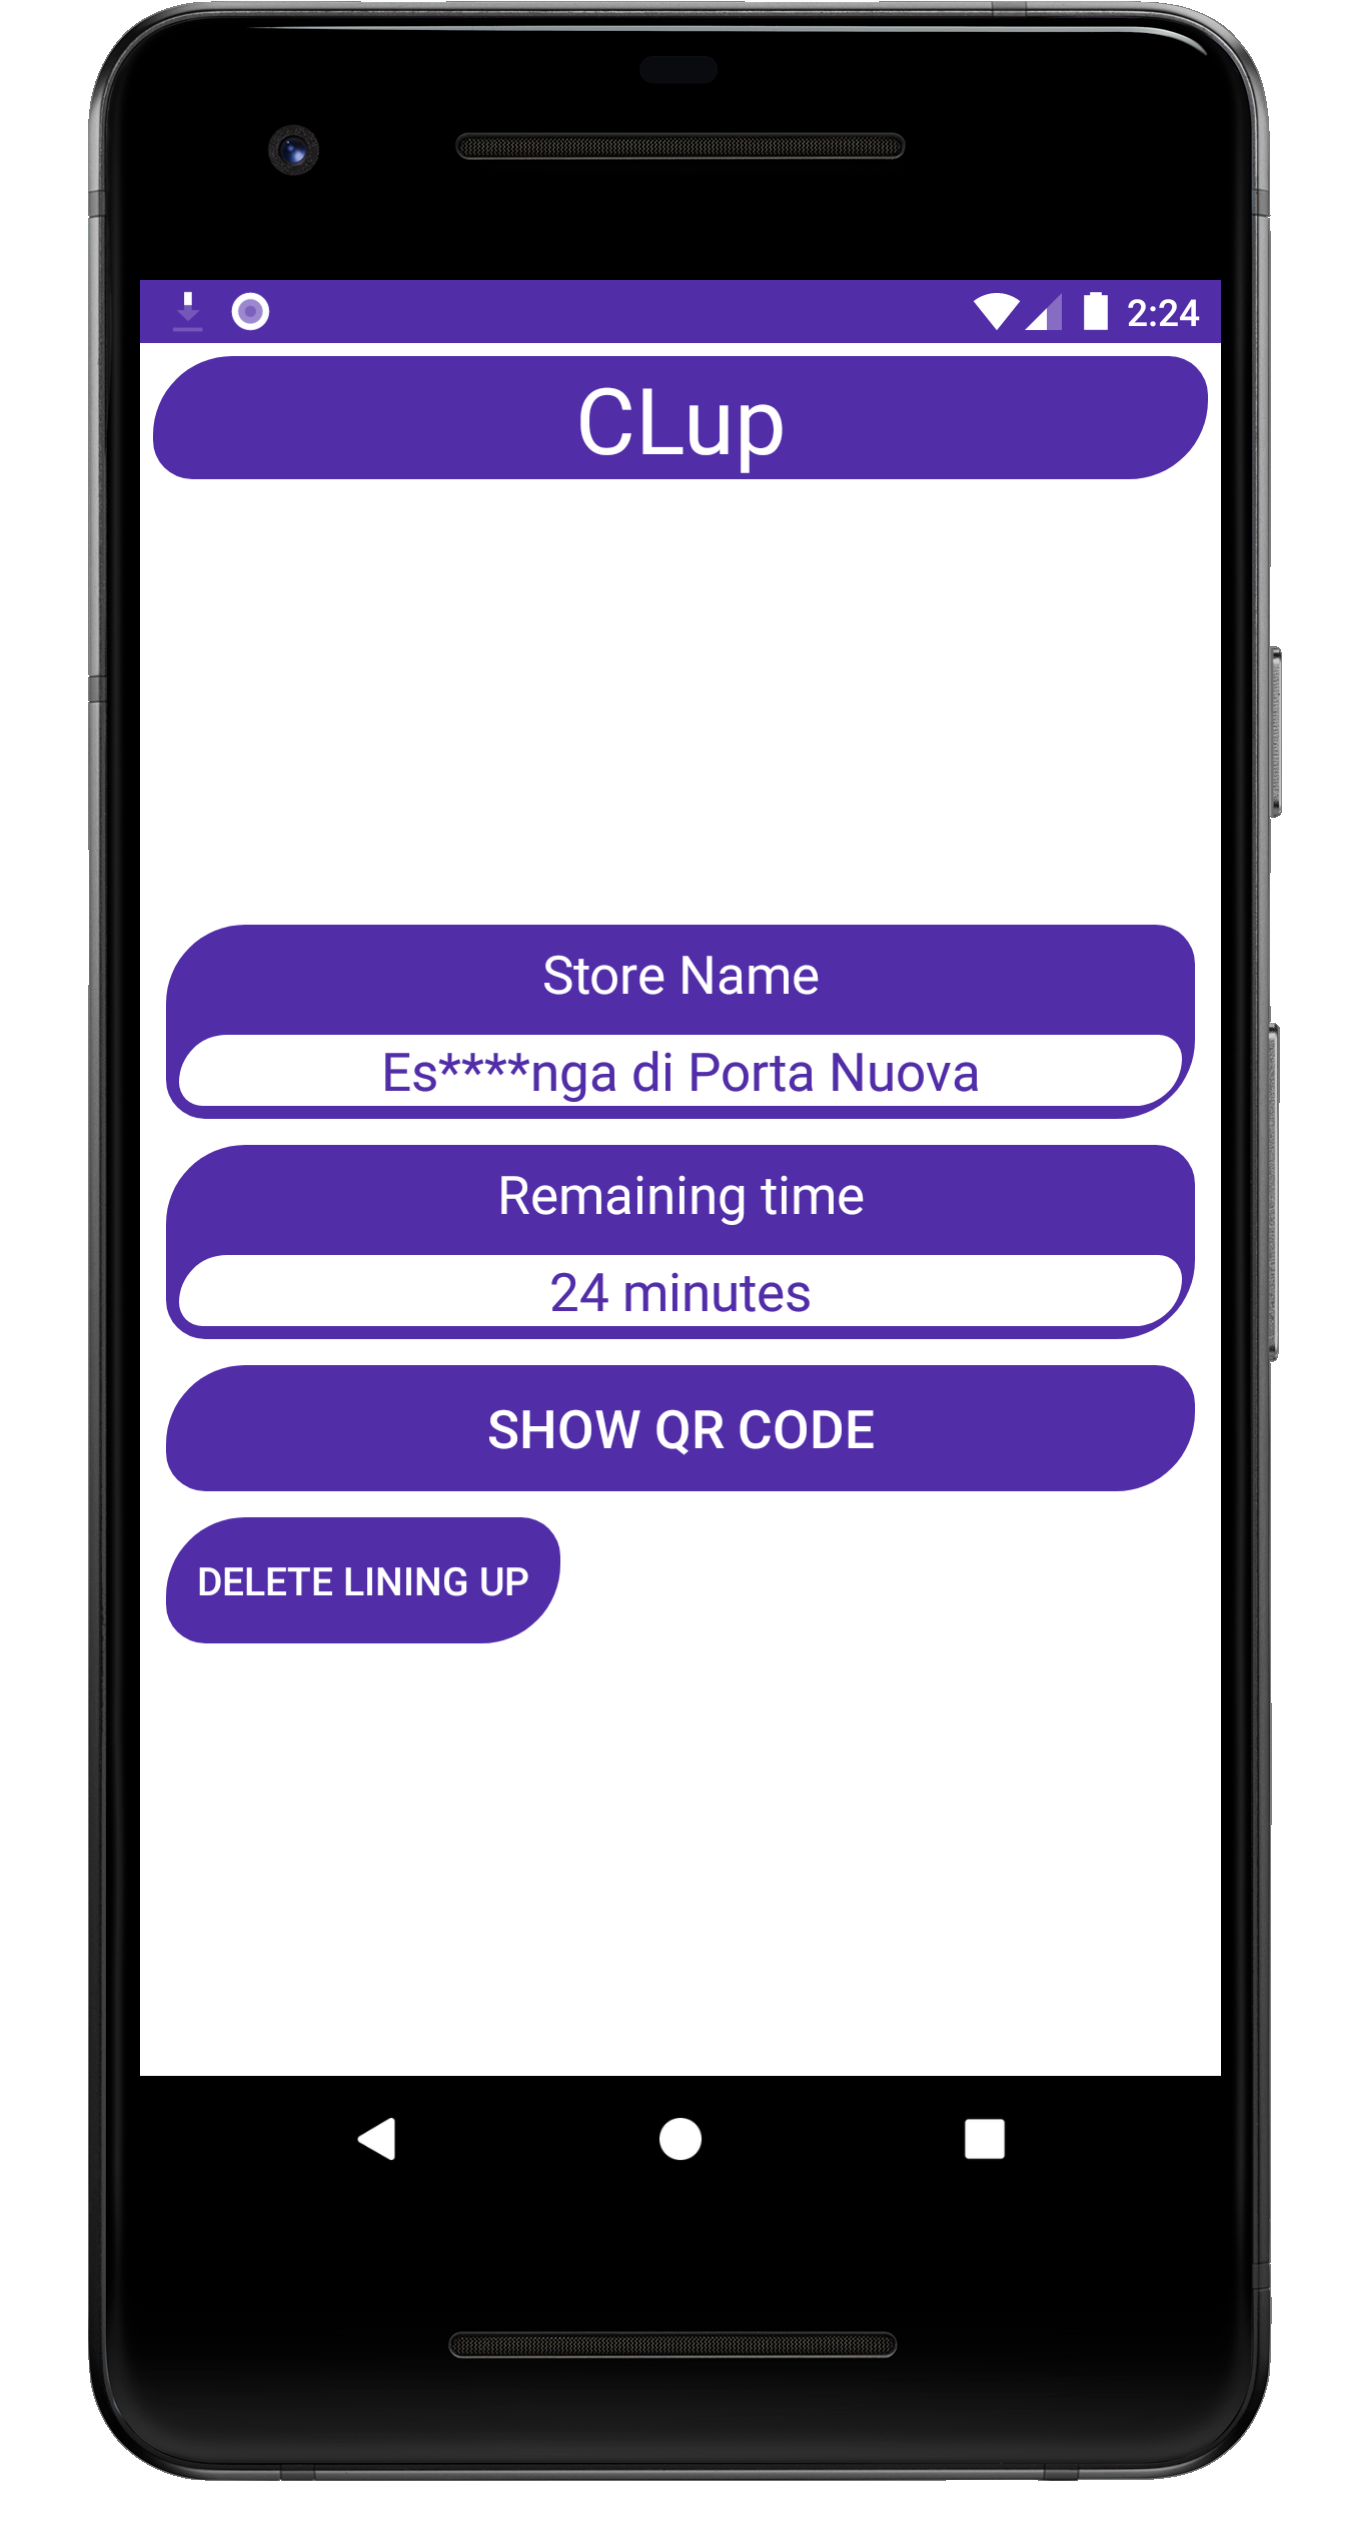
\includegraphics[width=0.3\textwidth]{images/get_status.png}}
	\subfigure[Show QR code page.]{\label{fig:ShowQRMockup}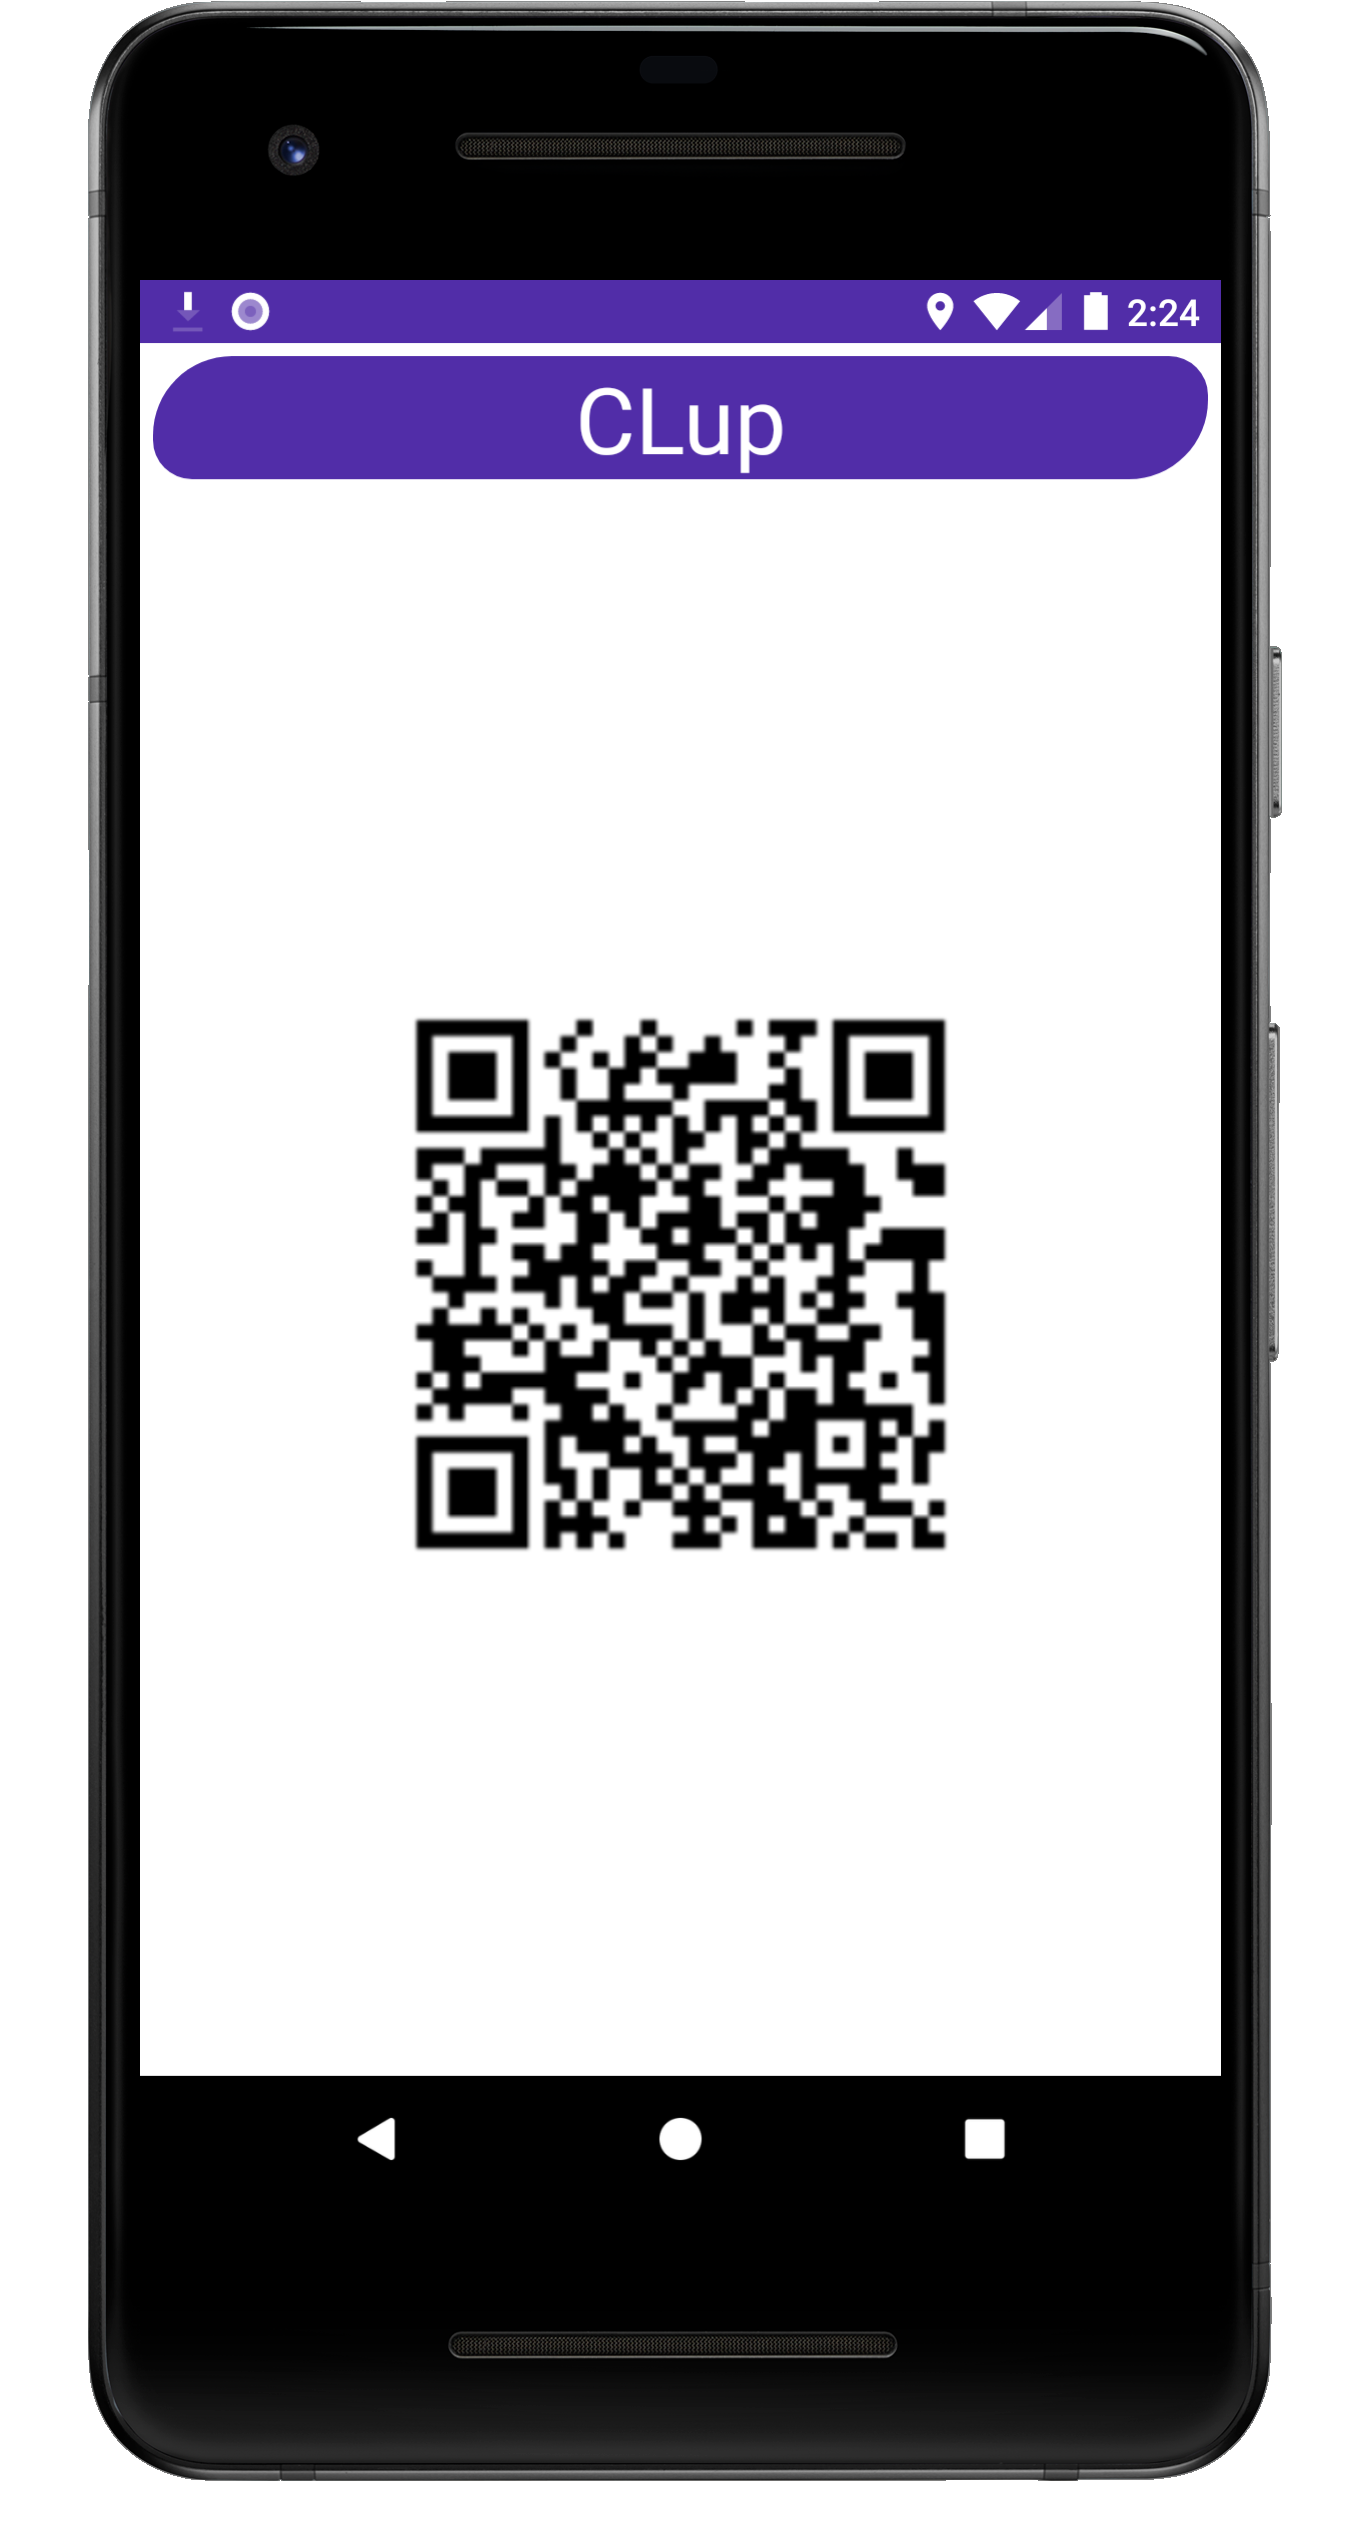
\includegraphics[width=0.3\textwidth]{images/show_qr_code.png}}
	\caption{Example of Status and Show QR code pages.}
\end{figure}

In figure~\ref{fig:ShowStatsMockup} has been reported a mockup showing a possible interface for the store manager to control the statistics about the status of the queue, instead,
in figure~\ref{fig:ControlQueueMockup} a page to control the parameters of the algorithm that schedules users and releases QR codes.


\begin{figure}[H]
	\centering     %%% not \center
	\subfigure[Show Stats page.]{\label{fig:ShowStatsMockup}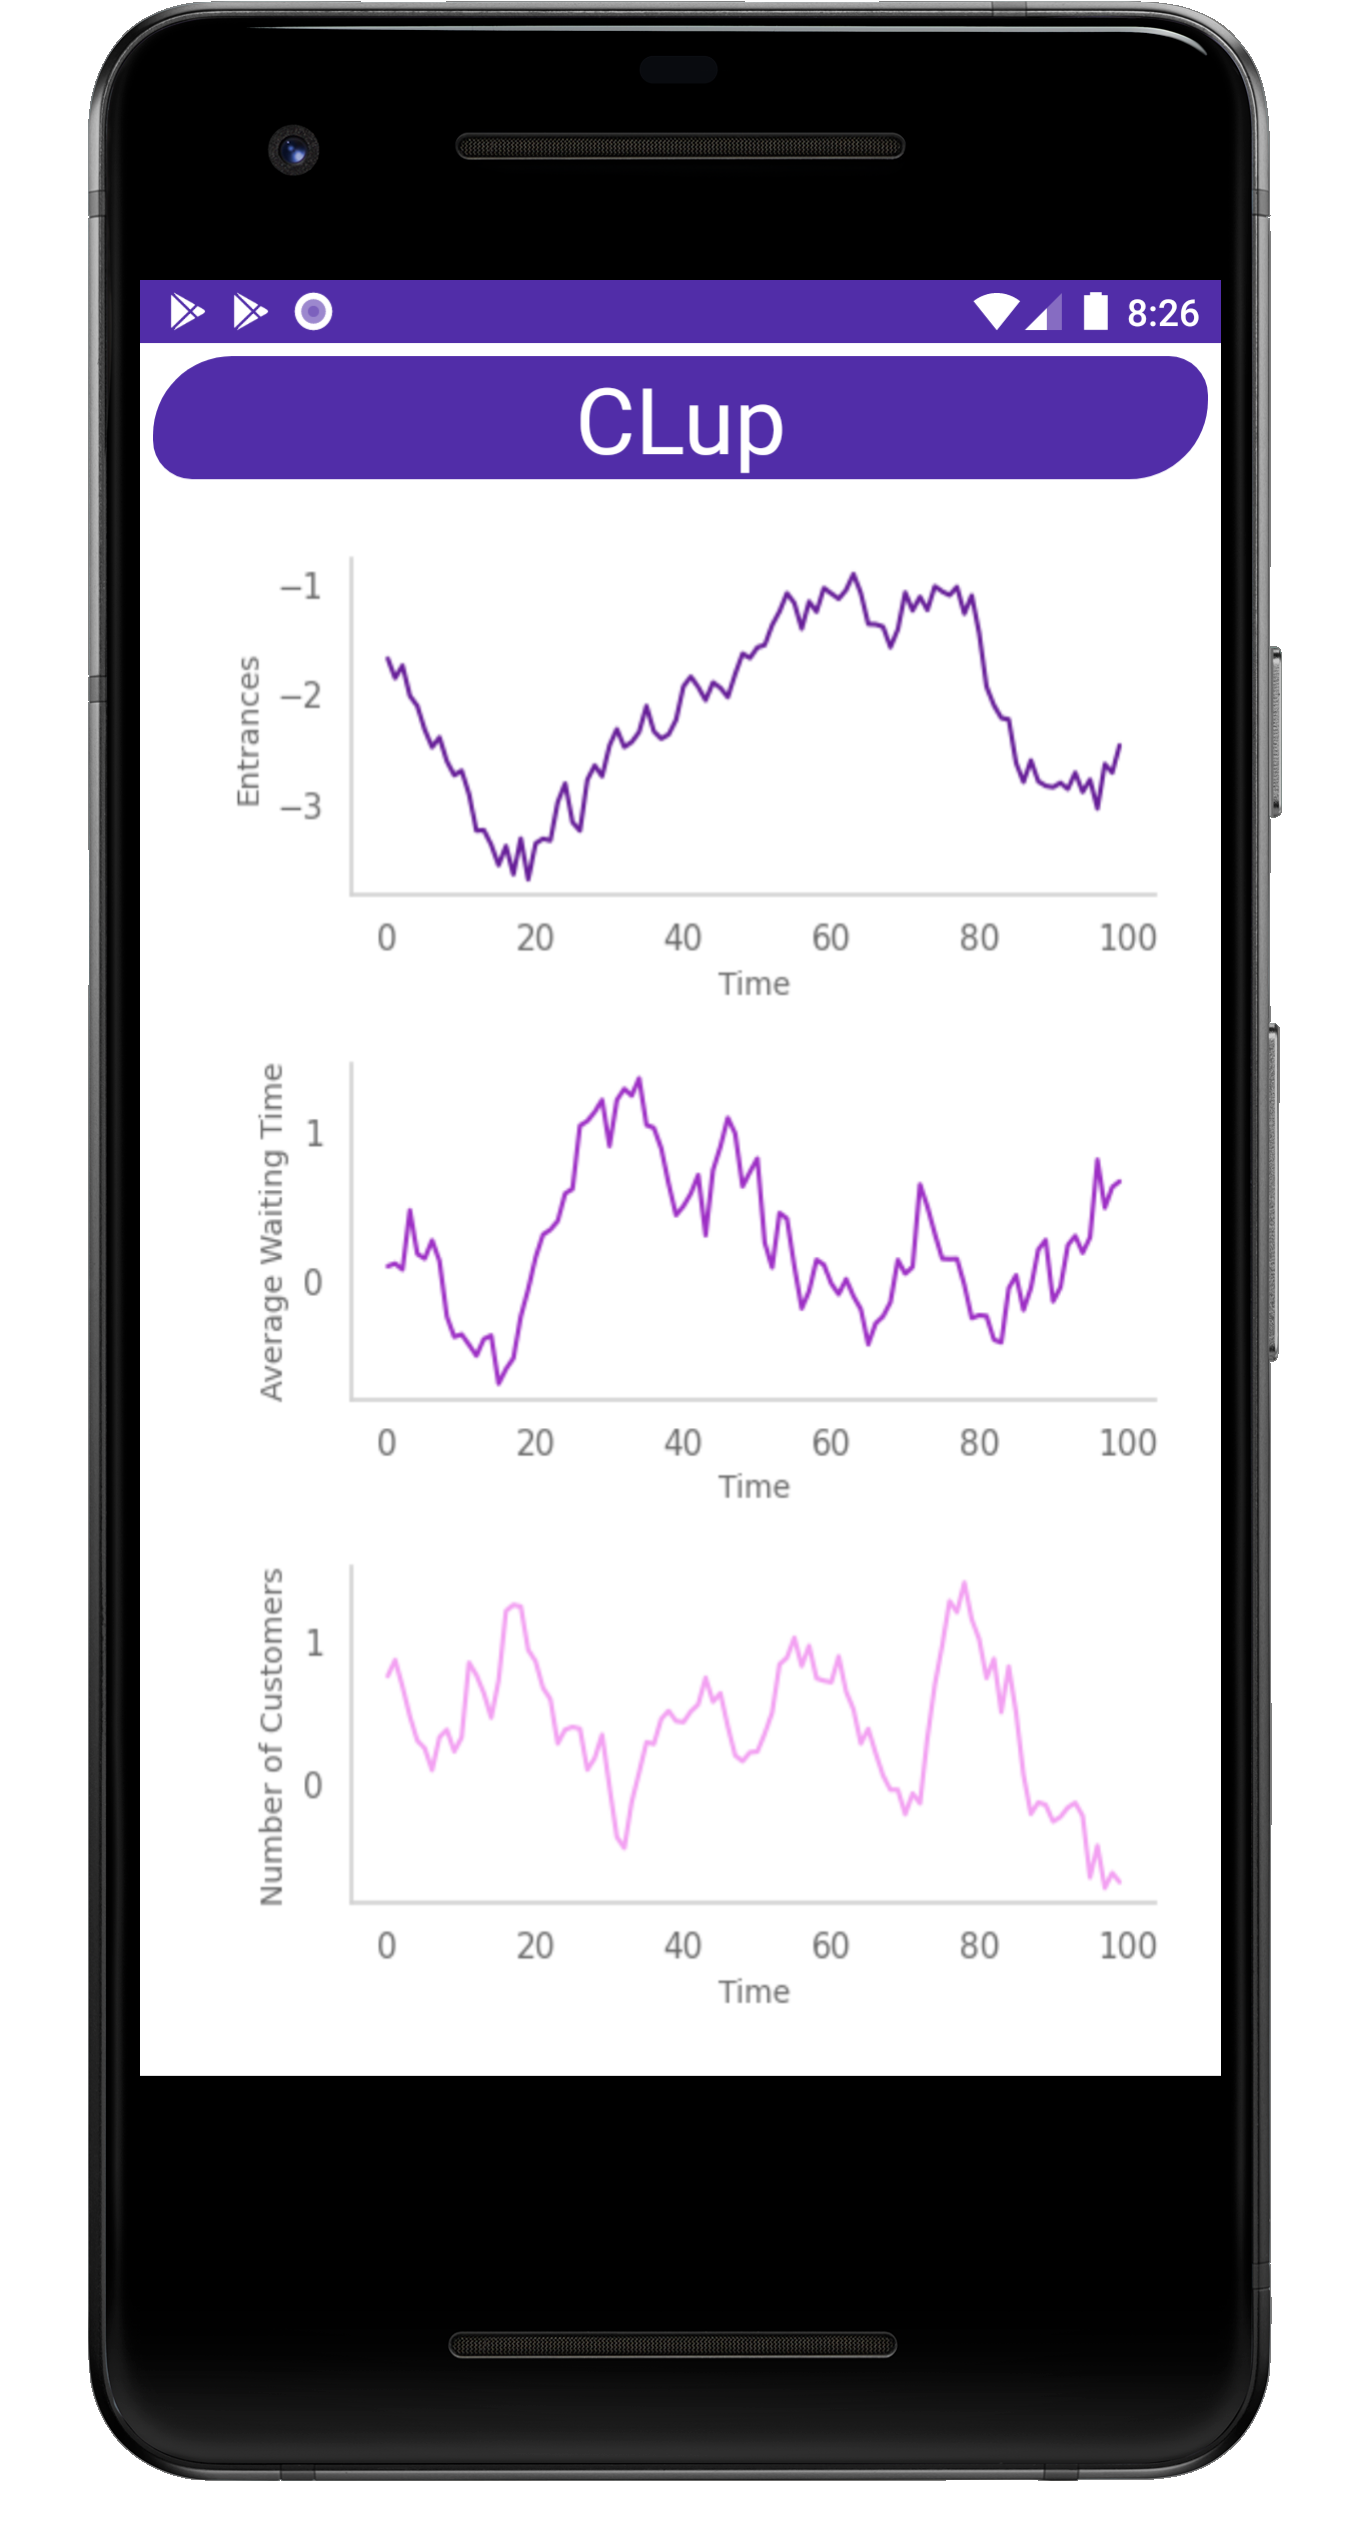
\includegraphics[width=0.3\textwidth]{images/show_stats.png}}
	\subfigure[Control Queue page.]{\label{fig:ControlQueueMockup}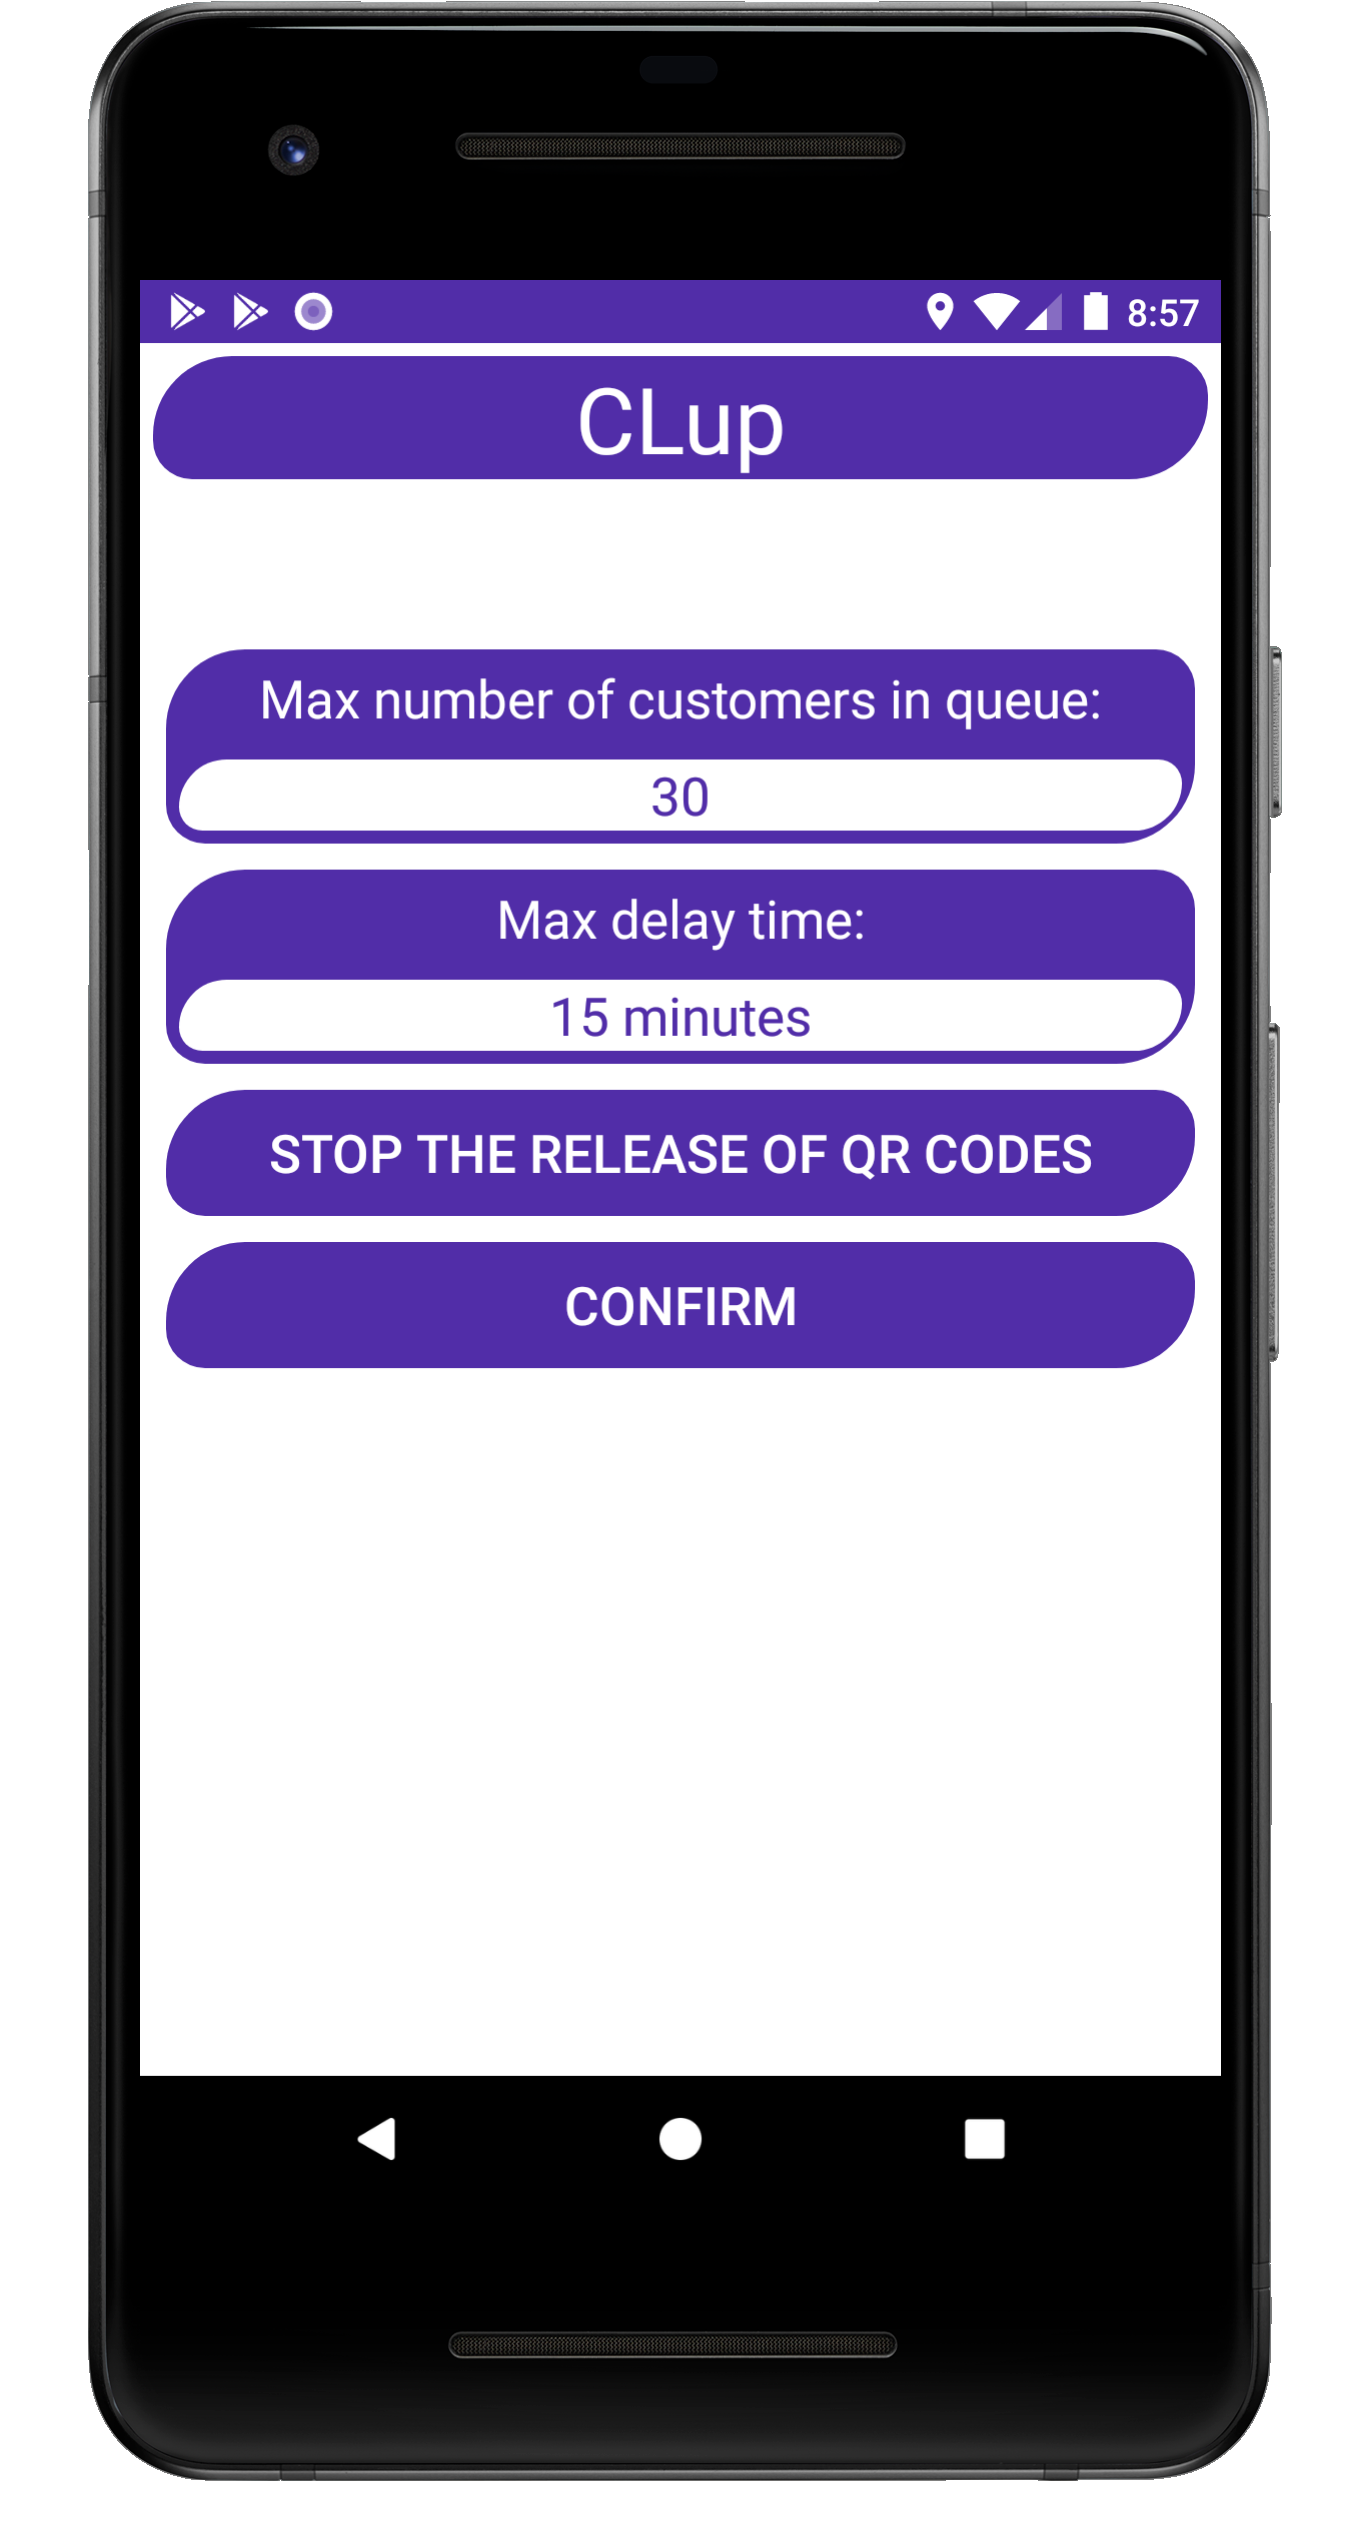
\includegraphics[width=0.3\textwidth]{images/control_queue.png}}
	\caption{Example of Show Stats and Control Queue pages.}
\end{figure}

\subsection{Hardware Interfaces}

The system is distributed over three main hardware resources.

\begin{itemize}
	\item \textbf{Smartphone}: used by the customers that wants to line up or book a visit from remote. The smartphone has to have a \gls{gps} module to send the position and an Internet connection active to receive live updates by the server.
	\item \textbf{Physical spot}: is a totem composed by a tablet and a printer. The printer is a peripheral of the tablet. The tablet must have an Internet connection active.
	\item \textbf{Turnstile}: is used to control the entries. The tablet of the store manager, the QR code scanner and the display, that shows the next ticket numbers, are parts of the turnstile. More precisely, turnstile, scanner and display are peripherals of the tablet.
	We can imagine the turnstile as the metal detector in the airports, in which the guards are seated on the opposite side of the entrance.
	The store manager controls everything by the tablet and the tablet controls the peripherals under the constraints imposed by the store manager and the remote server.
	Indeed the tablet has to have an Internet connection active.
\end{itemize}

\subsection{Software interfaces}

The system, to work properly, needs external \gls{api}.

\begin{itemize}
	\item \textbf{Store \glspl{api}}: are well-liked if they there are. Additional data provided by the store, such as the history of the purchases of the customers, can be used to improve the quality of the estimations of the residence time; the sections of the store that will be visited by customers and so on.
	\item \textbf{Google Maps \glspl{api}}: can be used to improve the estimation of the needed time to arrive to the store by the global position of the customer.
	\item \textbf{Google Firebase \glspl{api}}: to send live notifications to the customers.
\end{itemize}

\subsection{Communications Interfaces}

In this service we aren't scheduling to use external communications interfaces.
Only the standard Internet protocols.

\section{Functional Requirements}

\subsection{Scenarios}

Here we will describe some common scenarios of using the service.\\

\textbf{First scenario:}\\
Mario reads the newspaper and realize that the virus is a serious problem. He thinks that we should try to have behaviors that helps contain the problem, like take appointments on the spots we will go. He learns from Internet that the supermarket where he usually goes to, is using an application to take appointments, \gls{clup}. He registers himself, and from day on when he needs to do grocery shopping, he uses the application to digitally line-up. When the application notifies him that his turn is coming, he goes out in the directions of the supermarket. And only in few cases he found himself waiting few minutes to enter inside the store.\\

\textbf{Second scenario:}\\
Francesca usually goes on the same supermarket to do groceries, but for one reason or another she did not go there for two weeks. When she returned to that store, she learns that she needs to use an application to line up. She was told to download the application and to use it to line up, she did that and after she sign in. 
On the application she founds that there are shown some data like  the number of people before her, the time she needs to wait before entering the store, etc. 
Seeing that the waiting time is large she decided to go for a walk around the neighborhood and to return when the waiting time is of five minutes. She returned from her walk and saw that there was only a couple of people outside, she decided to wait and after few minutes she entered.\\

\textbf{Third Scenario:}\\
Maria is an old lady, she does not possess a smartphone but only an old phone that does not have Internet connection.
She decides to go to the supermarket in which a clerk tells her that she needs to use an application to line up. She explains to him that she does not have the means to do it and so, she is brought to the totem where she retrieves a ticket. She is recommended to stay close to the supermarket and to wait it there. During the chat with the clerk she also found that this mechanism is always guaranteed. 
Thanks to the fact that most people uses the application to line up, outside the store where the old lady is waiting, there are no crowds. Because all people either enter right away or at most they wait for few minutes, and so it reduces the risk for all.\\

\textbf{Fourth scenario:}\\
Andrea is a worker with a fixed schedule, every day he finishes to work at eight p.m., and so he has little time to do the groceries. He has tried to use the application \gls{clup} to line up, but he found himself, sometimes, with a waiting time of twenty minutes, without knowing what to do except to go to the store and wait outside. To try to solve this problem he used the book-a-visit function and took an appointment for the following day, choosing a schedule that worked for him, allowing him to arrive without hurry to the store. The next day he went to the store right on time and with a hint of amazement he entered right away. Impressed by the pleasant experience from that day on he started using regularly that function since it allows him to adjust it to his needs.\\


\textbf{Fifth scenario:}\\
Alfredo always uses the application to line up at the supermarket. One day he notices that when he lines up from his house the waiting time is always of twenty minutes even on the days where he goes there and see few people. With some reasoning he comes to the conclusion that the application gives him always a waiting time that is similar at the time he usually needs to get there. In fact, he really needs little less than twenty minutes to go there.\\


\textbf{Sixth scenario:}\\
Claudia is the manager of a supermarket that uses \gls{clup} and she checks the \gls{clup} to manage the flux of people inside the store. She always checks that the flux of people never reaches the eighty-five percent of the maximum capacity that the \gls{dpcm} imposed to the store, when there are not bookings and not more than ninety percent of the maximum capacity if there are some bookings that specify the department. 
One day even if the store respects these constrains, she notices that on one department, next to the entrance, a crowd is forming. Maybe it is happening because a recent sale on a category of products. She thinks that it would be appropriate to do not let other people enter until the problem is solved. So, she decides to use the application to temporarily block the number of new entrances. Leaving like that for few minutes the situation solve itself and she can allow again people to enter.\\


\subsection{Requirements}

In this section we report the requirements necessary to achieve our goals.

\subsection{Mapping}

\begin{table}[H]
\centering
\begin{tabular}{| m{0.2\textwidth} | m{0.8\textwidth} |} 
	\hline
	\textbf{Goal} &
		\textbf{G1: Keep customers in safe condition w.r.t the \gls{dpcm} in force inside the store.} \\
	\hline
	\textbf{Requirements} &
		\begin{itemize}
			\item {\textbf{[R1]}}: The system has to schedule entrances to the store.
			\item {\textbf{[R2]}}: The system has to compute the maximum capacity of the store w.r.t. the social distances imposed by the \gls{dpcm} in force.
			\item {\textbf{[R3]}}: The system has to monitor the customers residence time in the store.
			\item {\textbf{[R4]}}: The system has to allow authorized customers to enter in the store.
			\item {\textbf{[R5]}}: The system has to deny unauthorized customers to enter in the store.
			\item {\textbf{[R6]}}: The system has to know when a customer enters in the store.
			\item {\textbf{[R7]}}: The system has to know when a customer has left the store.
		\end{itemize} \\
	\hline
	\shortstack[l]{\textbf{Domain} \\ \textbf{Assumptions}} & 
		\begin{itemize}
			\item {\textbf{[D1]}}: There is a \gls{dpcm} in force.
			\item {\textbf{[D2]}}: Customers follow the rules imposed by the \gls{dpcm} in force.
			\item {\textbf{[D3]}}: Customers enter in the store only if the system authorizes them.
			\item {\textbf{[D4]}}: Customers don't stay in the shop longer than necessary and they go away from the store after they have done their shopping.
			% \item {\textbf{[D]}}: If customers booked a visit to the store and they specify the category of grocery, they won't buy other things.
		\end{itemize} \\ 
	\hline
\end{tabular}
\end{table}

\begin{table}[H]
\centering
\begin{tabular}{| m{0.2\textwidth} | m{0.8\textwidth} |} 
	\hline
	\textbf{Goal} &
		\textbf{G2: Limit the physical line situation in the proximity of the store} \\
	\hline
	\textbf{Requirements} &
		\begin{itemize}
			\item {\textbf{[R8]}}: The system has to estimate the residence time, of a customer, in the store.
			\item {\textbf{[R9]}}: The system has to infer the residence time of the customers based on past purchases.
			\item {\textbf{[R10]}}: The system has to estimate the time needed to arrive, to the store, from the position of the customer.
			\item {\textbf{[R11]}}: The system has to track the global position of the customers.
			\item {\textbf{[R12]}}: The system has to release QR codes to the customers.
			\item {\textbf{[R13]}}: The system has to allow store managers to limit the number of QR codes released.
			\item {\textbf{[R14]}}: The system has to allow the store manager to monitor the status of the queue.
			\item {\textbf{[R15]}}: The system has to notify customers about the remaining time to be authorized to enter in the store.
			\item {\textbf{[R16]}}: The system has to communicate which is the next served QR code number.
		\end{itemize} \\ 
	\hline
	\shortstack[l]{\textbf{Domain} \\ \textbf{Assumptions}} & 
		\begin{itemize}
			\item {\textbf{[D4]}}: Customers don't stay in the shop longer than necessary and they go away from the store after they have done their shopping.
			\item {\textbf{[D5]}}: Customers line up physically only if they have a valid (non expired) QR code.
			\item {\textbf{[D6]}}: Outside the store there is space to queue.
		\end{itemize} \\ 
	\hline
\end{tabular}
\end{table}

\begin{table}[H]
\centering
\begin{tabular}{| m{0.2\textwidth} | m{0.8\textwidth} |} 
	\hline
	\textbf{Goal} &
		\textbf{G3: Allow customers to line up from a remote device.} \\
		% requirements per l'app e il servizio di prenotazione (quality standard)
	\hline
	\textbf{Requirements} &
		\begin{itemize}
			\item {\textbf{[R17]}}: The system has to allow customers to register to the application.
			\item {\textbf{[R18]}}: The system has to allow users to login to the application.
			\item {\textbf{[R19]}}: The system has to release QR codes to the customers through the application.
			\item {\textbf{[R20]}}: The system has to alert customers if the queue is full.
			\item {\textbf{[R21]}}: The system has to encode the ticket number in the QR code.
			\item {\textbf{[R22]}}: The system has to allow customers to watch the QR code from the application.
			\item {\textbf{[R23]}}: The system has to allow customers to watch the ticket number encoded in the QR code.
			\item {\textbf{[R24]}}: The system has to allow customers to watch the remaining time to be authorized to enter in the store.
			\item {\textbf{[R25]}}: The system has to update the remaining time showed to the customers.
			\item {\textbf{[R26]}}: The system has to allow customers to delete a ticket.
			\item {\textbf{[R27]}}: The system has to notify customers about the validation status of the QR code.
			\item {\textbf{[R28]}}: The system has to check if users have Internet connection active.
			\item {\textbf{[R29]}}: The system has to check if users have allowed the permissions requested by the application.
		\end{itemize} \\ 
	\hline
	\shortstack[l]{\textbf{Domain} \\ \textbf{Assumptions}} & 
		\begin{itemize}
			\item {\textbf{[D7]}}: Customers have a smartphone.
			\item {\textbf{[D8]}}: Customers have installed the \gls{clup} application.
			\item {\textbf{[D9]}}: Users allow the permissions requested by the application.
			\item {\textbf{[D10]}}: Users keep Internet connection active.
		\end{itemize} \\ 
	\hline
\end{tabular}
\end{table}

\begin{table}[H]
\centering
\begin{tabular}{| m{0.2\textwidth} | m{0.8\textwidth} |} 
	\hline
	\textbf{Goal} &
		\textbf{G4: Allow store manager to monitor entrances.} \\
	\hline
	\textbf{Requirements} &
		\begin{itemize}
			\item {\textbf{[R30]}}: The system has to register store managers in the application.
			\item {\textbf{[R18]}}: The system has to allow users to login to the application.
			\item {\textbf{[R14]}}: The system has to allow store managers to monitor the status of the queue.
			\item {\textbf{[R13]}}: The system has to allow store managers to limit the number of QR codes released.
			\item {\textbf{[R31]}}: The system has to allow store managers to monitor the number of customers inside the store.
			\item {\textbf{[R32]}}: The system has to scan the QR codes of the customers.
			\item {\textbf{[R33]}}: The system has to allow store managers to modify the timing parameters of the scheduler.
			\item {\textbf{[R28]}}: The system has to check if users have Internet connection active.
			\item {\textbf{[R39]}}: The system has to check if users have allowed the permissions requested by the application.
		\end{itemize} \\ 
	\hline
	\shortstack[l]{\textbf{Domain} \\ \textbf{Assumptions}} & 
		\begin{itemize}
			\item {\textbf{[D9]}}: Users allow the permissions requested by the application.
			\item {\textbf{[D10]}}: Users keep Internet connection active.
			\item {\textbf{[D11]}}: There is a store manager present in the store.
		\end{itemize} \\ 
	\hline
\end{tabular}
\end{table}

\begin{table}[H]
\centering
\begin{tabular}{| m{0.2\textwidth} | m{0.8\textwidth} |} 
	\hline
	\textbf{Goal} &
		\textbf{G5: Allow customers to line up from a physical spot.} \\
	\hline
	\textbf{Requirements} &
		\begin{itemize}
			\item {\textbf{[R34]}}: The system has to allow unregistered customers to line up.
			\item {\textbf{[R35]}}: The system has to release QR codes from a physical spot.
			\item {\textbf{[R21]}}: The system has to encode the ticket number in the QR code.
			\item {\textbf{[R36]}}: The system has to print QR codes on a paper tickets.
			\item {\textbf{[R20]}}: The system has to alert customers if the queue is full.
			\item {\textbf{[R37]}}: The system has to alert when the paper and toner of the physical spot is going to finish.
		\end{itemize} \\ 
	\hline
	\shortstack[l]{\textbf{Domain} \\ \textbf{Assumptions}} & 
		\begin{itemize}
			\item {\textbf{[D12]}}: Physical spots are powered on every working day.
			\item {\textbf{[D13]}}: Physical spots are refilled when asked by the system. 
		\end{itemize} \\ 
	\hline
\end{tabular}
\end{table}

\begin{table}[H]
\centering
\begin{tabular}{| m{0.2\textwidth} | m{0.8\textwidth} |} 
	\hline
	\textbf{Goal} &
		\textbf{G6: Allow customers to book a visit from a remote device.} \\
		% requirements che implicano l'implementazione di una schermata nell'app per la prenotazione
	\hline
	\textbf{Requirements} &
		\begin{itemize}
			\item {\textbf{[R17]}}: The system has to allow customers to register to the application.
			\item {\textbf{[R18]}}: The system has to allow users to login to the application.
			\item {\textbf{[R38]}}: The system has to allow customers to specify the date and time for a visit to the store.
			\item {\textbf{[R39]}}: The system has to allow customers to specify the category of grocery they want to buy.
			\item {\textbf{[R19]}}: The system has to release QR codes to the customers through the application.
			\item {\textbf{[R20]}}: The system has to alert customers if the queue is full.
			\item {\textbf{[R21]}}: The system has to encode the ticket number in the QR code.
			\item {\textbf{[R22]}}: The system has to allow customers to watch the QR code from the application.
			\item {\textbf{[R23]}}: The system has to allow customers to watch the book-a-visit number encoded in the QR code.
			\item {\textbf{[R24]}}: The system has to allow customers to watch the remaining time to be authorized to enter in the store.
			\item {\textbf{[R26]}}: The system has to allow customers to delete a ticket.
			\item {\textbf{[R27]}}: The system has to notify customers about the validation status of the QR code.
			\item {\textbf{[R28]}}: The system has to check if users have Internet connection active.
			\item {\textbf{[R29]}}: The system has to check if users have allowed the permissions requested by the application.
		\end{itemize} \\ 
	\hline
	\shortstack[l]{\textbf{Domain} \\ \textbf{Assumptions}} & 
		\begin{itemize}
			\item {\textbf{[D7]}}: Customers have a smartphone.
			\item {\textbf{[D8]}}: Customers have installed the \gls{clup} application.
			\item {\textbf{[D9]}}: Users allow the permissions requested by the application.
			\item {\textbf{[D10]}}: Users keep Internet connection active.
		\end{itemize} \\ 
	\hline
\end{tabular}
\end{table}

\begin{table}[H]
\centering
\begin{tabular}{| m{0.2\textwidth} | m{0.4\textwidth} | m{0.4\textwidth} |} 
	\hline
		\textbf{Goal} & \textbf{Requirements} & \textbf{Domain Assumptions} \\
		\hline
		G1 & R1, R2, R3, R4, R5, R6, R7 & D1, D2, D3, D4 \\
		\hline
		G2 & R8, R9, R10, R11, R12, R13, R14, R15, R16 & D4, D5, D6 \\
		\hline
		G3 & R17, R18, R19, R20, R21, R22, R23, R24, R25, R26, R27, R28, R29 & D7, D8, D9, D10 \\
		\hline
		G4 & R13, R14, R18, R28, R30, R31, R32, R33, R39 & D9, D10, D11 \\
		\hline
		G5 & R20, R21, R34, R35, R36, R37 & D12, D13 \\
		\hline
		G6 & R17, R18, R19, R20, R21, R22, R23, R24, R26, R27, R28, R29, R38, R39 & D7, D8, D9, D10 \\
	\hline
\end{tabular}
\caption{Traceability matrix.}
\end{table}

\subsection{List of Requirements}

\begin{itemize}

	\item {\textbf{[R1]}}: The system has to schedule entrances to the store.
	\item {\textbf{[R2]}}: The system has to compute the maximum capacity of the store w.r.t. the social distances imposed by the \gls{dpcm} in force.
	\item {\textbf{[R3]}}: The system has to monitor the customers residence time in the store.
	\item {\textbf{[R4]}}: The system has to allow authorized customers to enter in the store.
	\item {\textbf{[R5]}}: The system has to deny unauthorized customers to enter in the store.
	\item {\textbf{[R6]}}: The system has to know when a customer enters in the store.
	\item {\textbf{[R7]}}: The system has to know when a customer has left the store.
	\item {\textbf{[R8]}}: The system has to estimate the residence time, of a customer, in the store.
	\item {\textbf{[R9]}}: The system has to infer the residence time of the customers based on past purchases.
	\item {\textbf{[R10]}}: The system has to estimate the time needed to arrive, to the store, from the position of the customer.
	\item {\textbf{[R11]}}: The system has to track the global position of the customers.
	\item {\textbf{[R12]}}: The system has to release QR codes to the customers.
	\item {\textbf{[R13]}}: The system has to allow store managers to limit the number of QR codes released.
	\item {\textbf{[R14]}}: The system has to allow the store manager to monitor the status of the queue.
	\item {\textbf{[R15]}}: The system has to notify customers about the remaining time to be authorized to enter in the store.
	\item {\textbf{[R16]}}: The system has to communicate which is the next served QR code number.
	\item {\textbf{[R17]}}: The system has to allow customers to register to the application.
	\item {\textbf{[R18]}}: The system has to allow users to login to the application.
	\item {\textbf{[R19]}}: The system has to release QR codes to the customers through the application.
	\item {\textbf{[R20]}}: The system has to alert customers if the queue is full.
	\item {\textbf{[R21]}}: The system has to encode the ticket number in the QR code.
	\item {\textbf{[R22]}}: The system has to allow customers to watch the QR code from the application.
	\item {\textbf{[R23]}}: The system has to allow customers to watch the ticket number encoded in the QR code.
	\item {\textbf{[R24]}}: The system has to allow customers to watch the remaining time to be authorized to enter in the store.
	\item {\textbf{[R25]}}: The system has to update the remaining time showed to the customers.
	\item {\textbf{[R26]}}: The system has to allow customers to delete a ticket.
	\item {\textbf{[R27]}}: The system has to notify customers about the validation status of the QR code.
	\item {\textbf{[R28]}}: The system has to check if users have Internet connection active.
	\item {\textbf{[R29]}}: The system has to check if users have allowed the permissions requested by the application.
	\item {\textbf{[R30]}}: The system has to register store managers in the application.
	\item {\textbf{[R31]}}: The system has to allow store managers to monitor the number of customers inside the store.
	\item {\textbf{[R32]}}: The system has to scan the QR codes of the customers.
	\item {\textbf{[R33]}}: The system has to allow store managers to modify the timing parameters of the scheduler.
	\item {\textbf{[R34]}}: The system has to allow unregistered customers to line up.
	\item {\textbf{[R35]}}: The system has to release QR codes from a physical spot.
	\item {\textbf{[R36]}}: The system has to print QR codes on a paper tickets.
	\item {\textbf{[R37]}}: The system has to alert when the paper and toner of the physical spot is going to finish.
	\item {\textbf{[R38]}}: The system has to allow customers to specify the date and time for a visit to the store.
	\item {\textbf{[R39]}}: The system has to allow customers to specify the category of grocery they want to buy.

\end{itemize}

\subsection{Definition of Use Case Diagrams}


\begin{figure}[H]
	\centering
	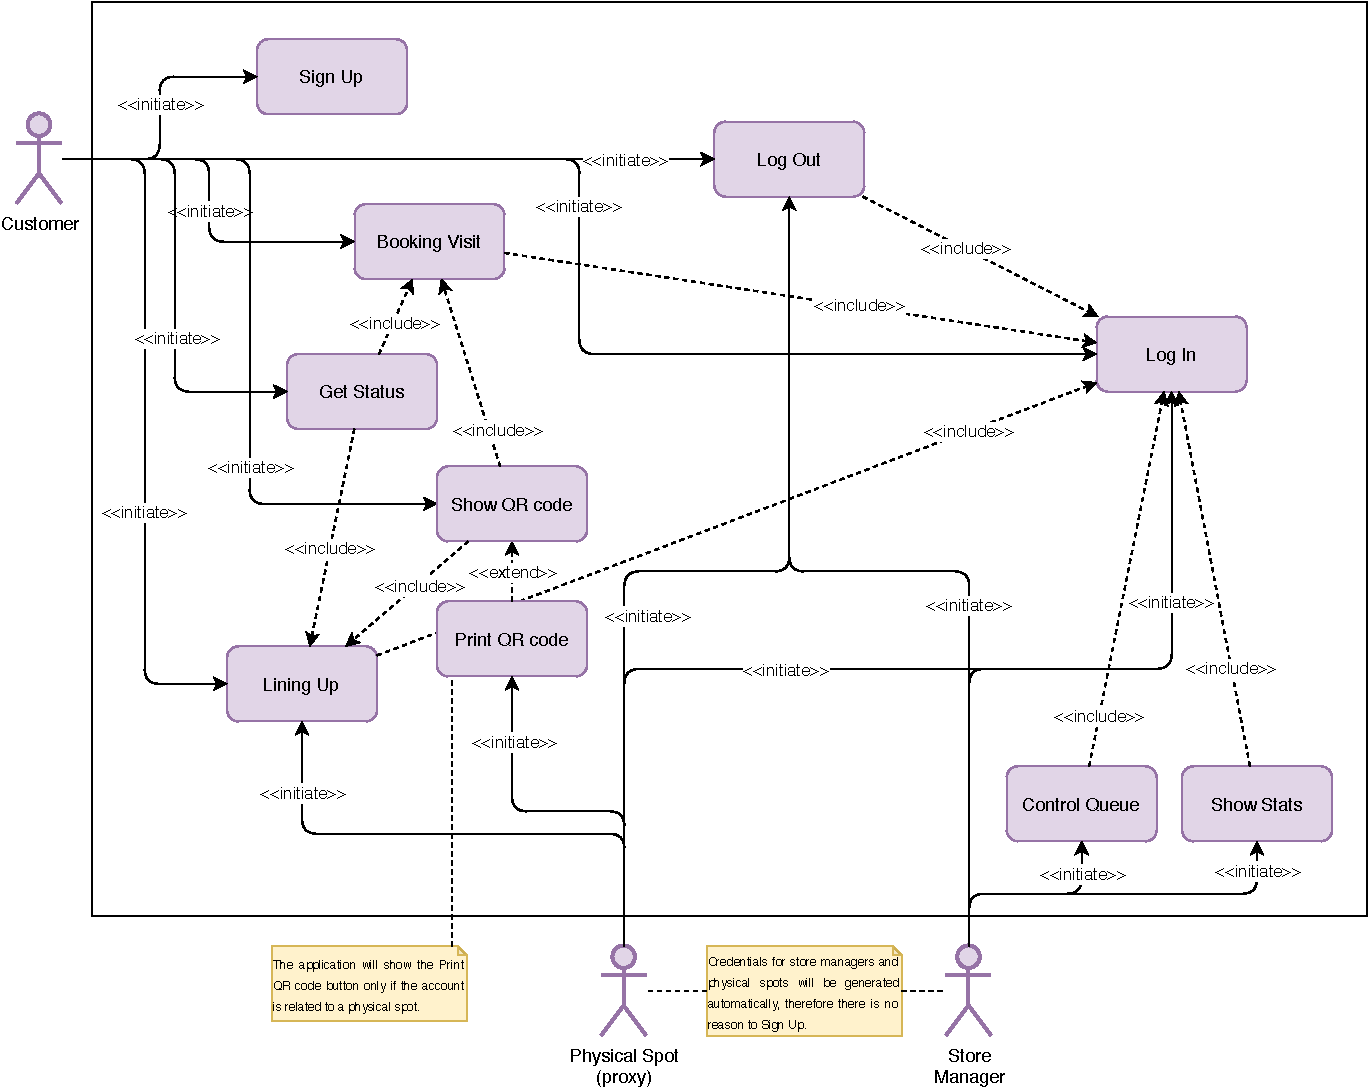
\includegraphics[width=1.0\textwidth]{images/use_cases_diagram.pdf}
	\caption{Use cases diagram.}
\end{figure}

\begin{table}[H]
\centering
\begin{tabular}{| m{0.3\textwidth} | m{0.7\textwidth} |} 
	\hline
	\textbf{Name} & Sign Up \\ 
	\hline
	\textbf{Actor} & Customer \\ 
	\hline
	\textbf{Entry Conditions} & Customer is on the Sign Up page. \\ 
	\hline
	\textbf{Event Flows} &
	\begin{itemize}
		\item Customer inserts the requested information in the form.
		\item Customer clicks on the Sign Up button.
	\end{itemize} \\ 
	\hline
	\textbf{Exit Conditions} & Sign Up completed successfully and customer is logged in, then the application shows the Home page. \\ 
	\hline
	\textbf{Exceptions} &
	\begin{itemize}
		\item Customer's username already in use.
		\item Empty form field.
		\item Policy agreement rejected.
		\item Lost Internet connection.
	\end{itemize} \\ 
	\hline
\end{tabular}
\caption{Customer - use case: \textbf{Sign Up}.}
\label{tableSignUp}
\end{table}

\begin{table}[H]
\centering
\begin{tabular}{| m{0.3\textwidth} | m{0.7\textwidth} |} 
	\hline
	\textbf{Name} & Log In \\ 
	\hline
	\textbf{Actor} & Customer - Physical Spot - Store Manager \\ 
	\hline
	\textbf{Entry Conditions} & Actor is on the Log In page. \\ 
	\hline
	\textbf{Event Flows} &
	\begin{itemize}
	\item Actor inserts the requested information in the form.
	\item Actor clicks on the Log In button.
	\end{itemize} \\ 
	\hline
	\textbf{Exit Conditions} & Log In completed successfully and actor is redirected to the Home page. \\ 
	\hline
	\textbf{Exceptions} &
	\begin{itemize}
	\item Actor's username or password incorrect.
	\item Empty form field.
	\item Lost Internet connection.
	\end{itemize} \\ 
	\hline
\end{tabular}
\caption{Use case: \textbf{Log In}.}
\label{tableLogIn}
\end{table}

\begin{table}[H]
\centering
\begin{tabular}{| m{0.3\textwidth} | m{0.7\textwidth} |} 
	\hline
	\textbf{Name} & Log Out \\ 
	\hline
	\textbf{Actor} & Customer - Physical Spot - Store Manager \\ 
	\hline
	\textbf{Entry Conditions} & Actor is on the Log Out page. \\ 
	\hline
	\textbf{Event Flows} &
	\begin{itemize}
	\item Actor clicks on the Log Out button.
	\end{itemize} \\ 
	\hline
	\textbf{Exit Conditions} & Log Out completed successfully and actor is redirected to the Log In page. \\ 
	\hline
	\textbf{Exceptions} &
	\begin{itemize}
	\item Actor already logged out.
	\item Lost Internet connection.
	\end{itemize} \\ 
	\hline
\end{tabular}
\caption{Use case: \textbf{Log Out}.}
\label{tableLogOut}
\end{table}

\begin{table}[H]
\centering
\begin{tabular}{| m{0.3\textwidth} | m{0.7\textwidth} |} 
	\hline
	\textbf{Name} & Lining Up \\ 
	\hline
	\textbf{Actor} & Customer - Physical Spot \\ 
	\hline
	\textbf{Entry Conditions} & Actor is on the Home page. \\ 
	\hline
	\textbf{Event Flows} &
	\begin{itemize}
	\item Actor clicks on the Lining Up button.
	\item Actor inserts the requested data in the form.
	\item Actor clicks on the confirmation button.
	\end{itemize} \\ 
	\hline
	\textbf{Exit Conditions} & Lining Up completed successfully, the application returns the Status page. \\ 
	\hline
	\textbf{Exceptions} &
	\begin{itemize}
	\item Previous Lining Up action was not expired (only in case of remote customer).
	\item Previous Booking Visit action was not expired (only in case of remote customer).
	\item Actor wasn't logged.
	\item Lost Internet connection.
	\end{itemize} \\ 
	\hline
\end{tabular}
\caption{Use case: \textbf{Lining Up}.}
\label{tableLiningUp}
\end{table}

\begin{table}[H]
\centering
\begin{tabular}{| m{0.3\textwidth} | m{0.7\textwidth} |} 
	\hline
	\textbf{Name} & Booking Visit \\ 
	\hline
	\textbf{Actor} & Customer \\ 
	\hline
	\textbf{Entry Conditions} & Customer is on the Home page. \\ 
	\hline
	\textbf{Event Flows} &
	\begin{itemize}
	\item Customer clicks on the Booking Visit button.
	\item Customer fills the form with the requested data.
	\item Customer clicks on the Submit button.
	\end{itemize} \\ 
	\hline
	\textbf{Exit Conditions} & Booking Visit completed successfully and the application returns, to the customer, the Status page. \\ 
	\hline
	\textbf{Exceptions} &
	\begin{itemize}
	\item Previous Lining Up action was not expired.
	\item Previous Booking Visit action was not expired.
	\item Customer wasn't logged.
	\item Lost Internet connection.
	\end{itemize} \\ 
	\hline
\end{tabular}
\caption{Customer - use case: \textbf{Booking Visit}.}
\label{tableBookingVisit}
\end{table}

\begin{table}[H]
\centering
\begin{tabular}{| m{0.3\textwidth} | m{0.7\textwidth} |} 
	\hline
	\textbf{Name} & Show QR code - Print QR code \\ 
	\hline
	\textbf{Actor} & Customer - Physical Spot \\ 
	\hline
	\textbf{Entry Conditions} & Actor is on the Home page. \\ 
	\hline
	\textbf{Event Flows} &
	\begin{itemize}
	\item Actor clicks on the Show QR (Print QR) code button.
	\end{itemize} \\ 
	\hline
	\textbf{Exit Conditions} & The application shows (print) the QR code. \\ 
	\hline
	\textbf{Exceptions} &
	\begin{itemize}
	\item QR code wasn't saved on the application correctly (only in case of remote customer).
	\item No Lining Up, or Booking Visit, action previously performed (only in case of remote customer).
	\item Actor wasn't logged.
	\item Spot finished the paper.
	\item Spot finished the ink.
	\end{itemize} \\ 
	\hline
\end{tabular}
\caption{Use case: \textbf{Show QR code - Print QR code}.}
\label{tableShowQR}
\end{table}

\begin{table}[H]
\centering
\begin{tabular}{| m{0.3\textwidth} | m{0.7\textwidth} |} 
	\hline
	\textbf{Name} & Get Status \\ 
	\hline
	\textbf{Actor} & Customer \\ 
	\hline
	\textbf{Entry Conditions} & Customer is on the Home page. \\ 
	\hline
	\textbf{Event Flows} &
	\begin{itemize}
	\item Customer clicks on the Get Status button.
	\end{itemize} \\ 
	\hline
	\textbf{Exit Conditions} & The application returns the Get Status page showing information about the last Lining Up, or Booking Visit, operation. \\ 
	\hline
	\textbf{Exceptions} &
	\begin{itemize}
	\item No operation previously performed, therefore there is no data to show.
	\item Customer wasn't logged.
	\item Lost Internet connection.
	\end{itemize} \\ 
	\hline
\end{tabular}
\caption{Customer - use case: \textbf{Get Status}.}
\label{tableGetStatus}
\end{table}

\begin{table}[H]
\centering
\begin{tabular}{| m{0.3\textwidth} | m{0.7\textwidth} |} 
	\hline
	\textbf{Name} & Control Queue \\ 
	\hline
	\textbf{Actor} & Store Manager \\ 
	\hline
	\textbf{Entry Conditions} & Store Manager is on the Home page. \\ 
	\hline
	\textbf{Event Flows} &
	\begin{itemize}
	\item Store Manager clicks on the Control Queue button.
	\end{itemize} \\ 
	\hline
	\textbf{Exit Conditions} & The application returns the Control Queue page showing options to manage the queue. \\ 
	\hline
	\textbf{Exceptions} &
	\begin{itemize}
	\item Store Manager wasn't logged.
	\item Lost Internet connection.
	\end{itemize} \\ 
	\hline
\end{tabular}
\caption{Store Manager - use case: \textbf{Control Queue}.}
\label{tableGetStatus}
\end{table}

\begin{table}[H]
\centering
\begin{tabular}{| m{0.3\textwidth} | m{0.7\textwidth} |} 
	\hline
	\textbf{Name} & Show Stats \\ 
	\hline
	\textbf{Actor} & Store Manager \\ 
	\hline
	\textbf{Entry Conditions} & Store Manager is on the Home page. \\ 
	\hline
	\textbf{Event Flows} &
	\begin{itemize}
	\item Store Manager clicks on the Show Stats button.
	\end{itemize} \\ 
	\hline
	\textbf{Exit Conditions} & The application returns the Show Stats page showing information about the number of customers inside the store, the length of the queue and other information about the waiting time in queue. \\ 
	\hline
	\textbf{Exceptions} &
	\begin{itemize}
	\item Store Manager wasn't logged.
	\item Lost Internet connection.
	\end{itemize} \\ 
	\hline
\end{tabular}
\caption{Store Manager - use case: \textbf{Show Stats}.}
\label{tableGetStatus}
\end{table}


\subsection{Use Cases and Sequence/Activity Diagrams}

\begin{figure}[H]
	\centering
	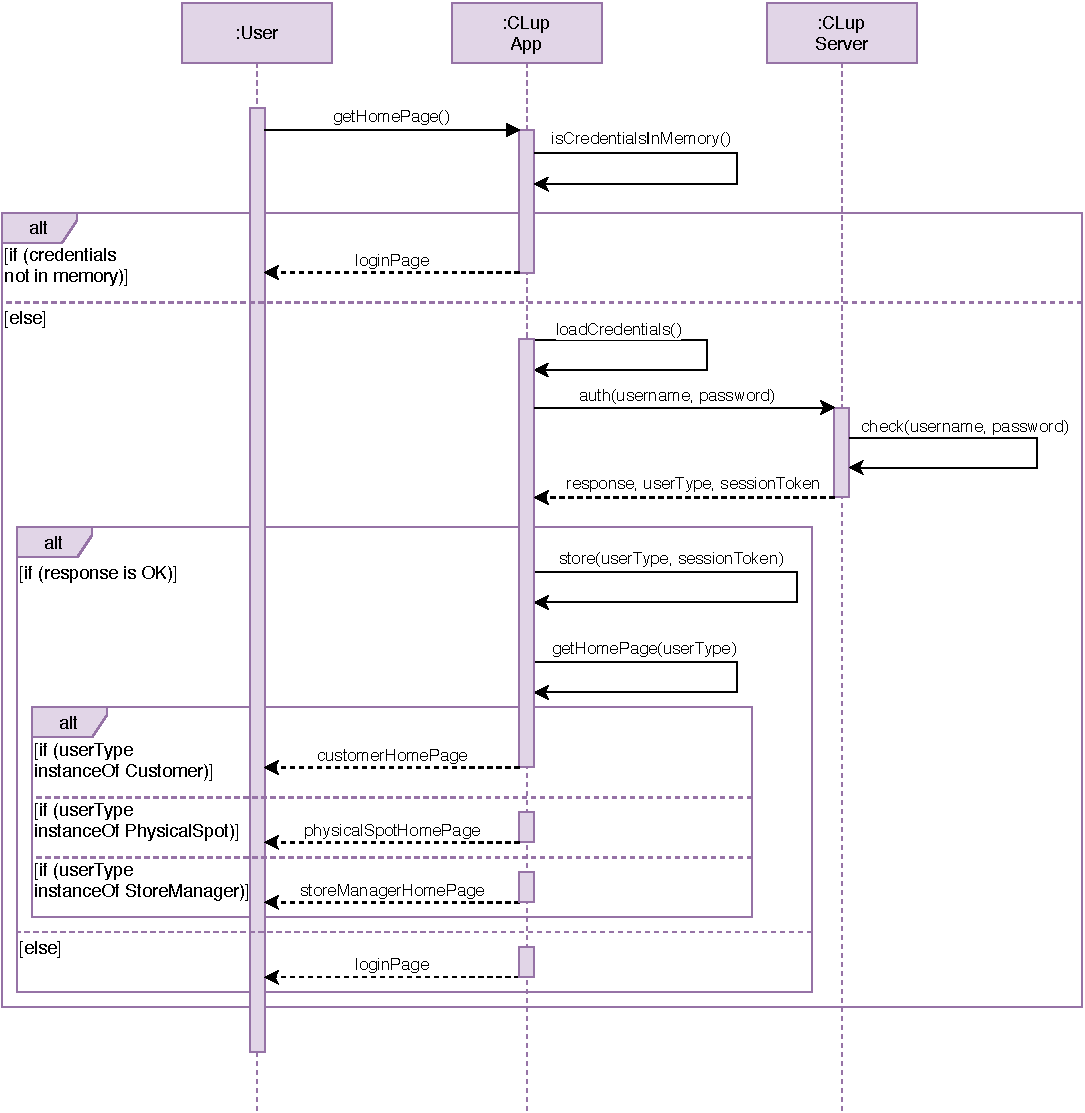
\includegraphics[width=1.0\textwidth]{images/getHomePage_sequence_diagram.pdf}
	\caption{Home page sequence diagram.}
\end{figure}

\begin{figure}[H]
	\centering
	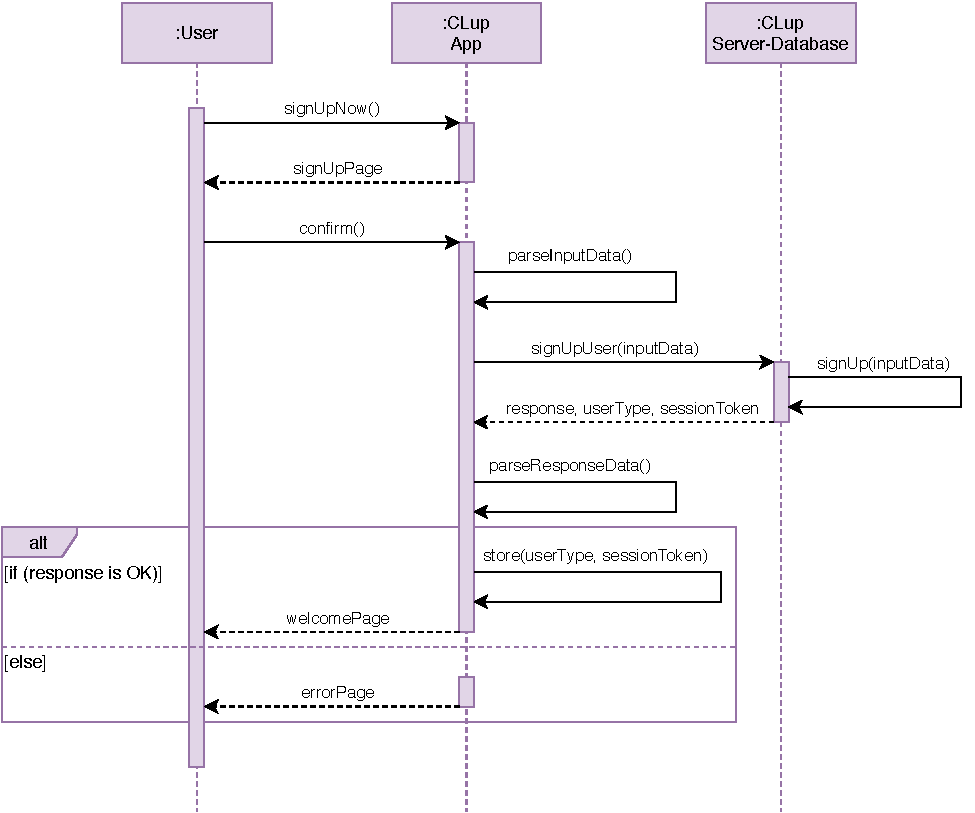
\includegraphics[width=1.0\textwidth]{images/signUp_sequence_diagram.pdf}
	\caption{Sign Up sequence diagram.}
\end{figure}

\begin{figure}[H]
	\centering
	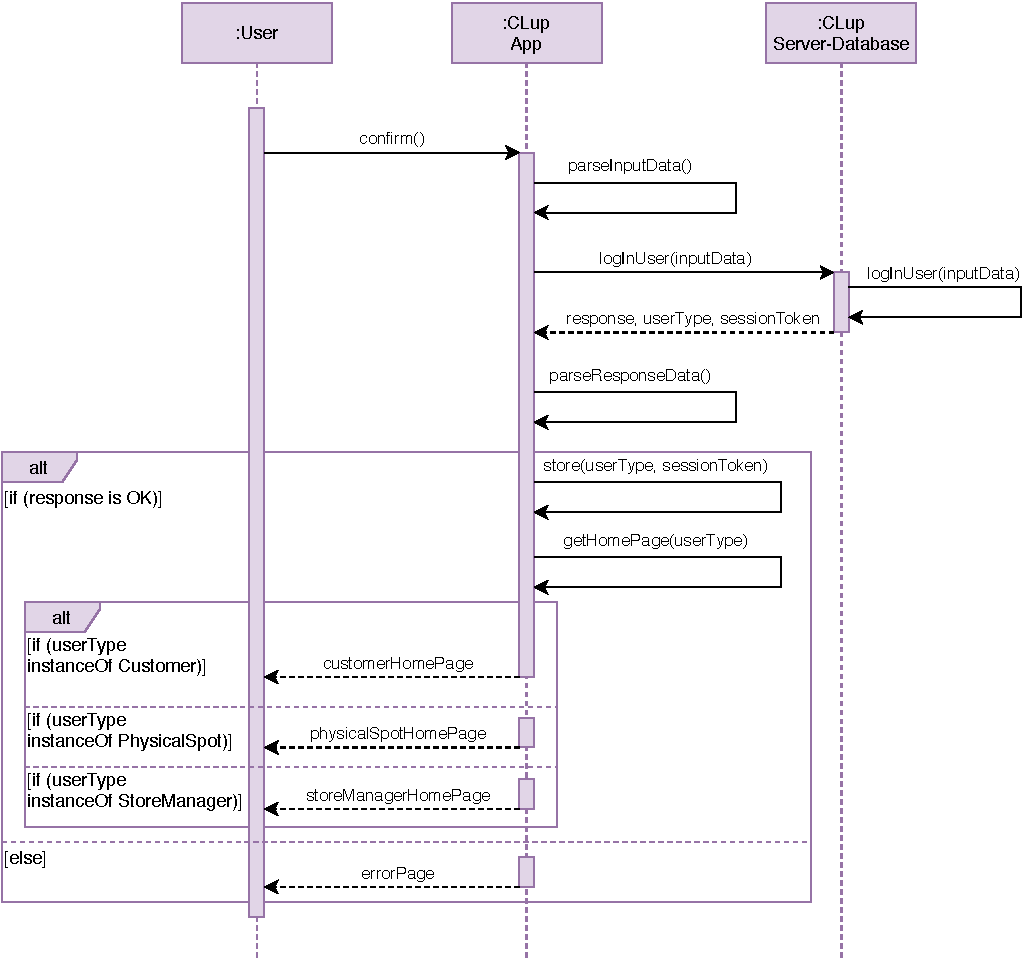
\includegraphics[width=1.0\textwidth]{images/logIn_sequence_diagram.pdf}
	\caption{Log In sequence diagram.}
\end{figure}

\begin{figure}[H]
	\centering
	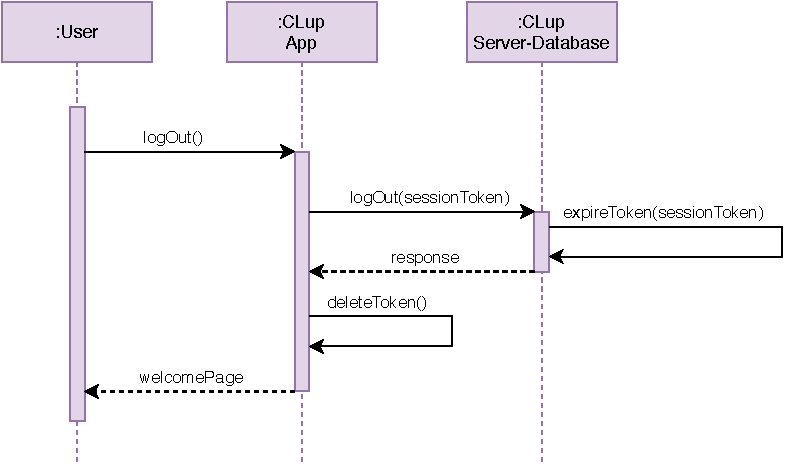
\includegraphics[width=1.0\textwidth]{images/logOut_sequence_diagram.pdf}
	\caption{Log Out sequence diagram.}
\end{figure}

\begin{figure}[H]
	\centering
	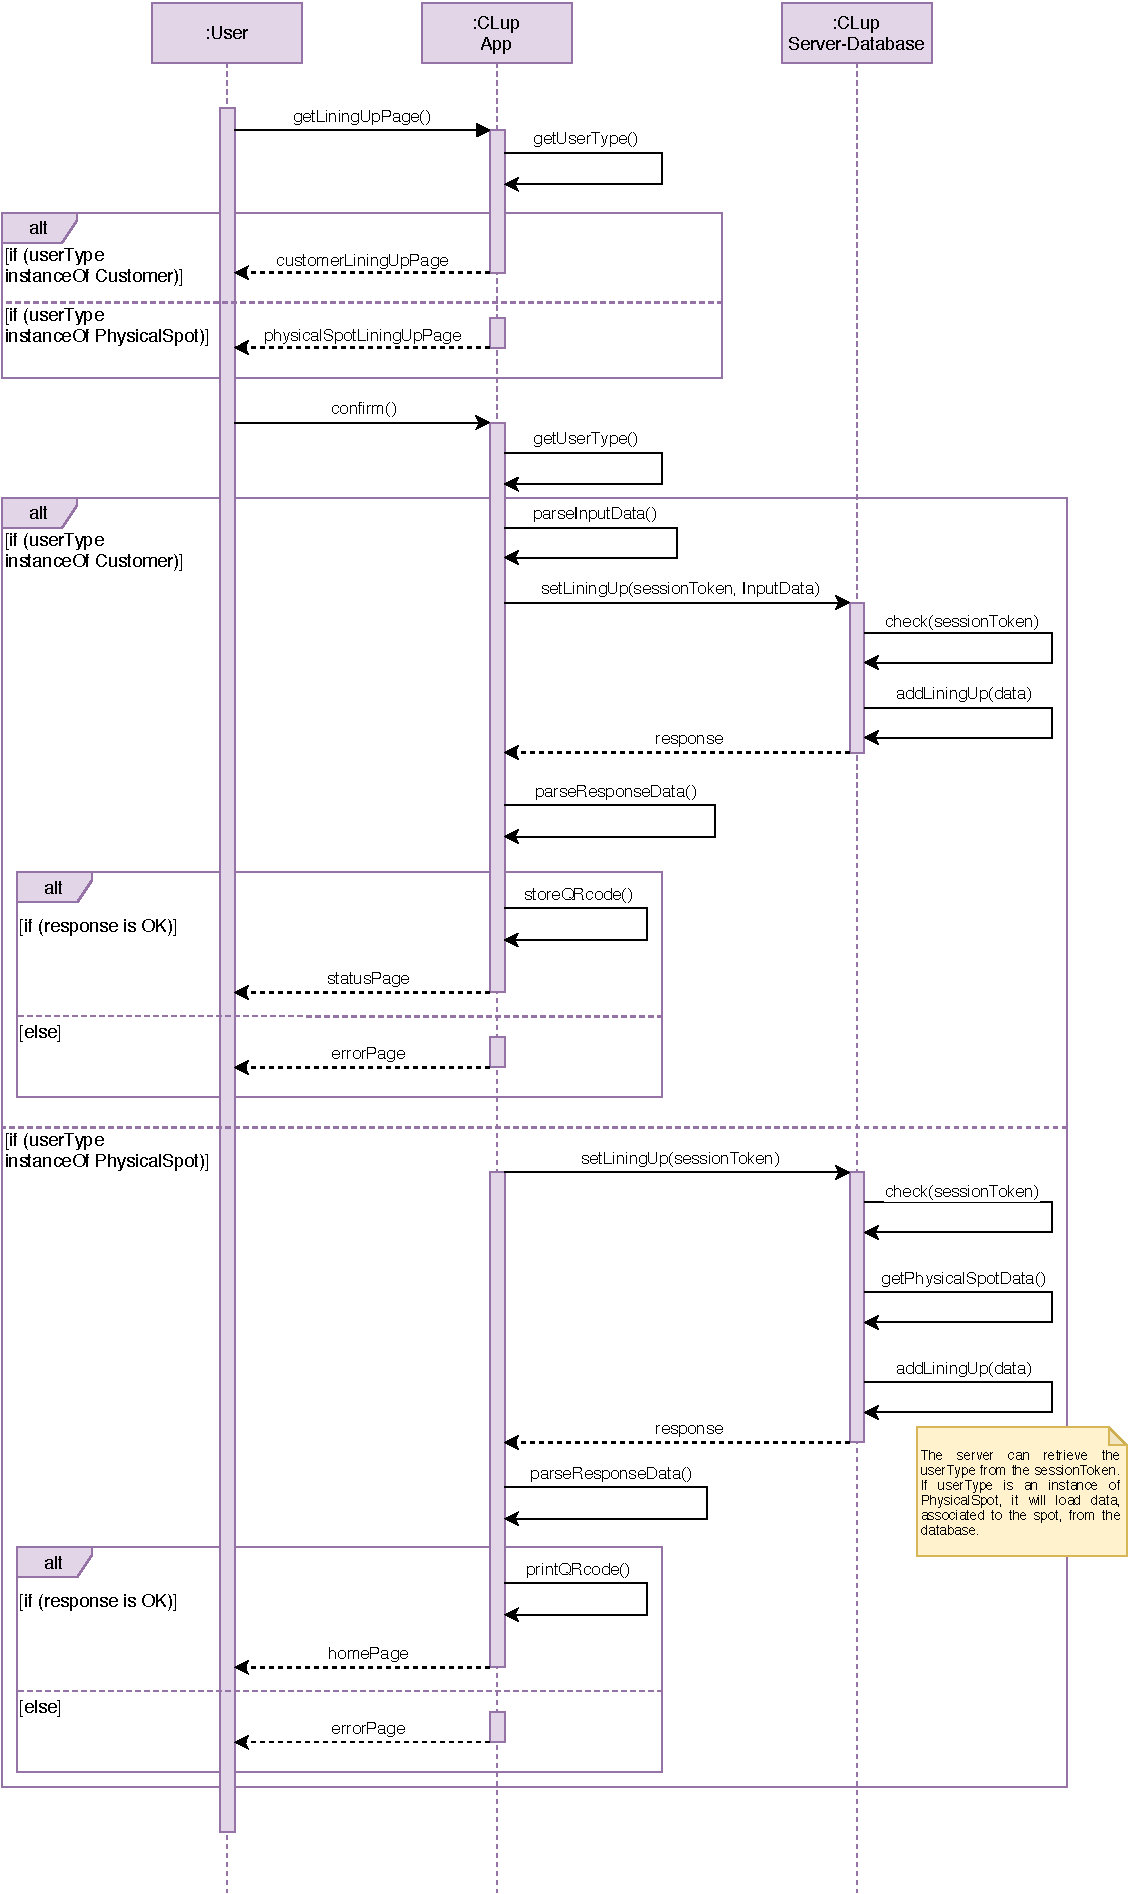
\includegraphics[width=1.0\textwidth]{images/liningUp_sequence_diagram.pdf}
	\caption{Lining Up sequence diagram.}
	\label{figure:liningUpSequenceDiagram}
\end{figure}

\begin{figure}[H]
	\centering
	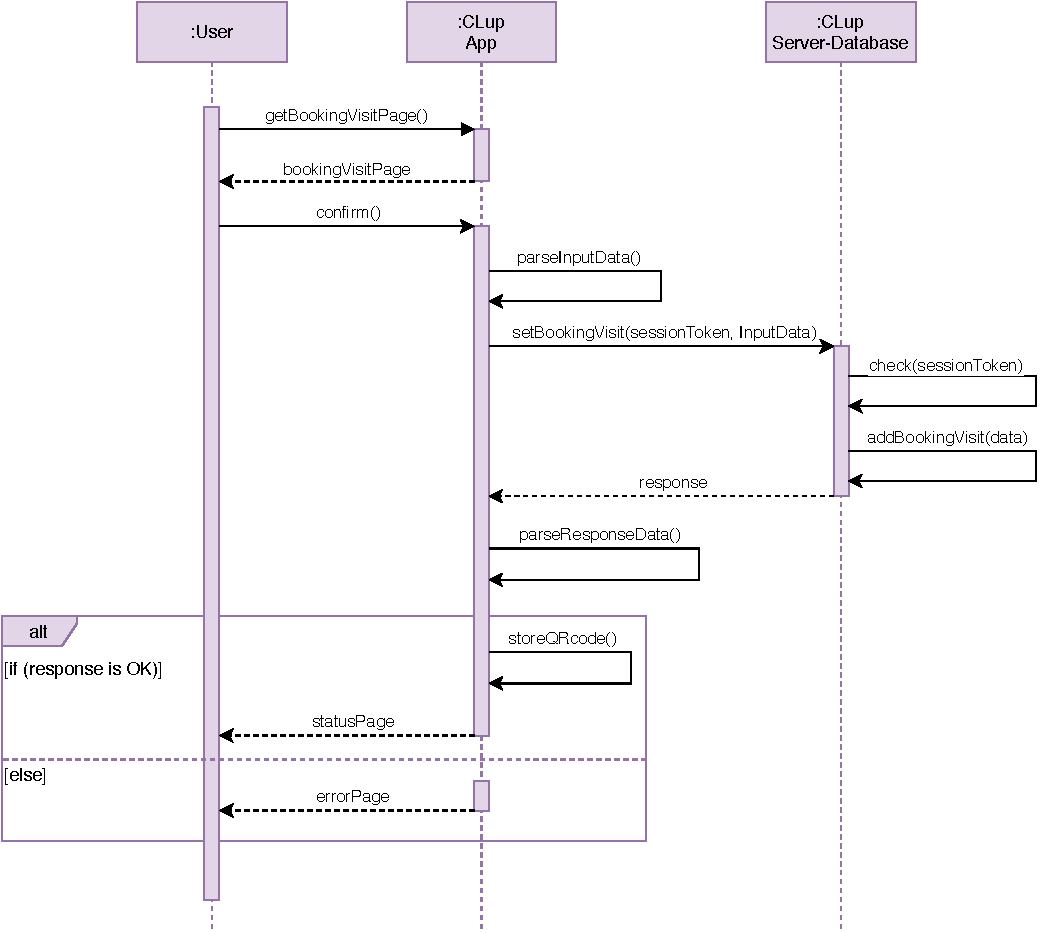
\includegraphics[width=1.0\textwidth]{images/bookingVisit_sequence_diagram.pdf}
	\caption{Booking a Visit sequence diagram.}
\end{figure}

\begin{figure}[H]
	\centering
	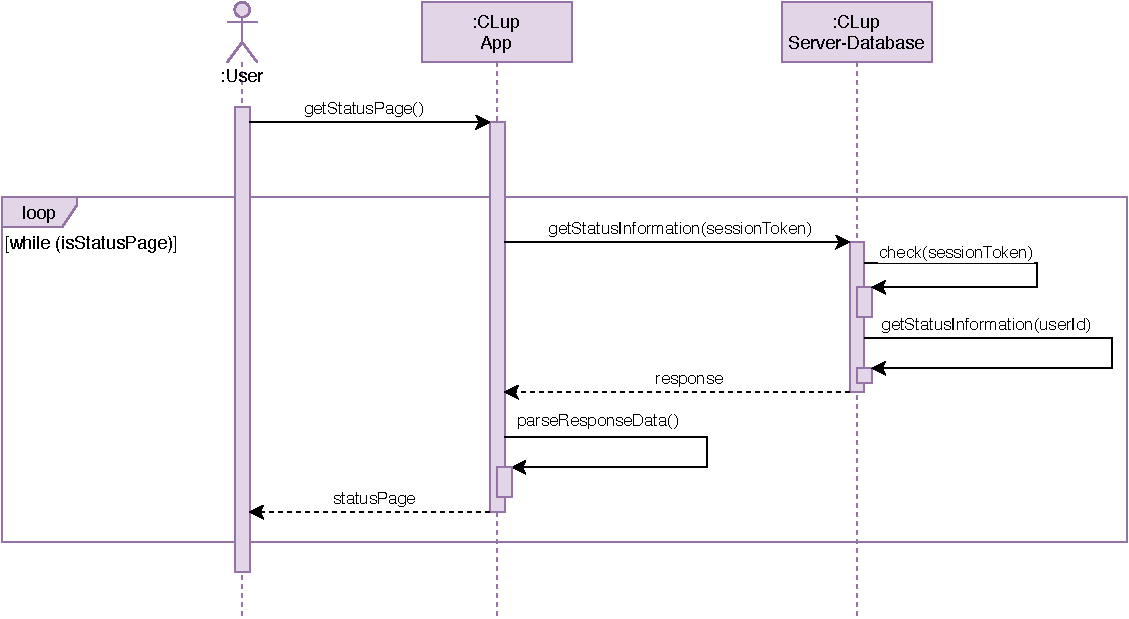
\includegraphics[width=1.0\textwidth]{images/getStatusPage_sequence_diagram.pdf}
	\caption{Get Status sequence diagram.}
\end{figure}

\begin{figure}[H]
	\centering
	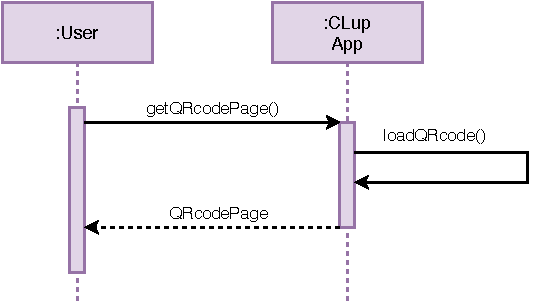
\includegraphics[width=1.0\textwidth]{images/getQRcodePage_sequence_diagram.pdf}
	\caption{QR code page sequence diagram.}
\end{figure}

\begin{figure}[H]
	\centering
	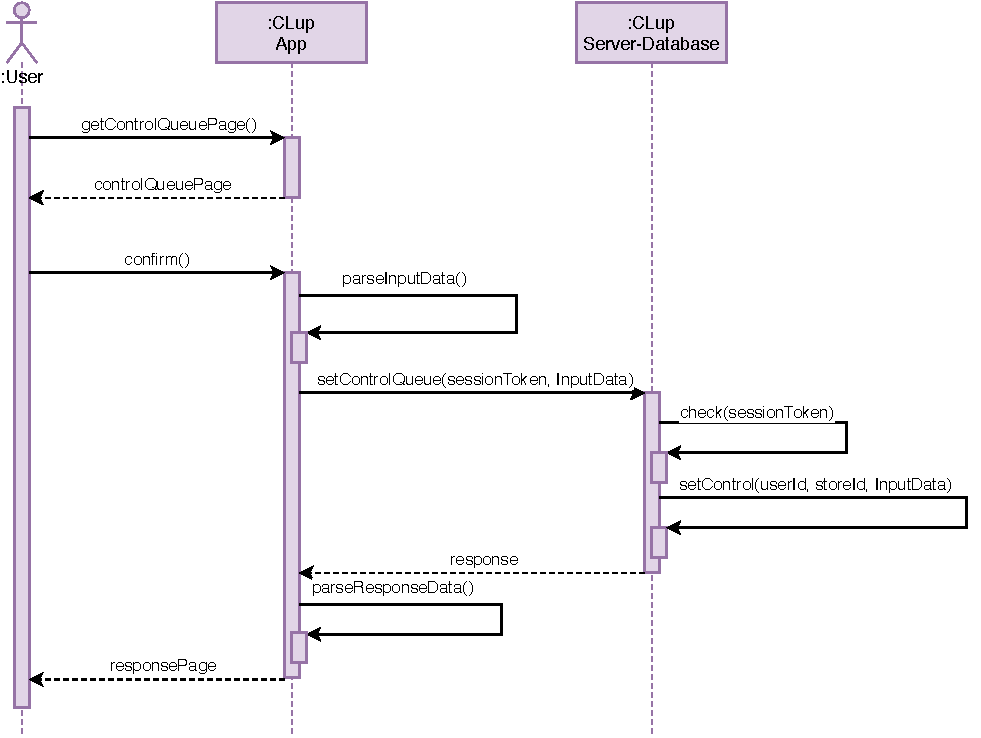
\includegraphics[width=1.0\textwidth]{images/getControlQueuePage_sequence_diagram.pdf}
	\caption{Control Queue sequence diagram.}
\end{figure}

\begin{figure}[H]
	\centering
	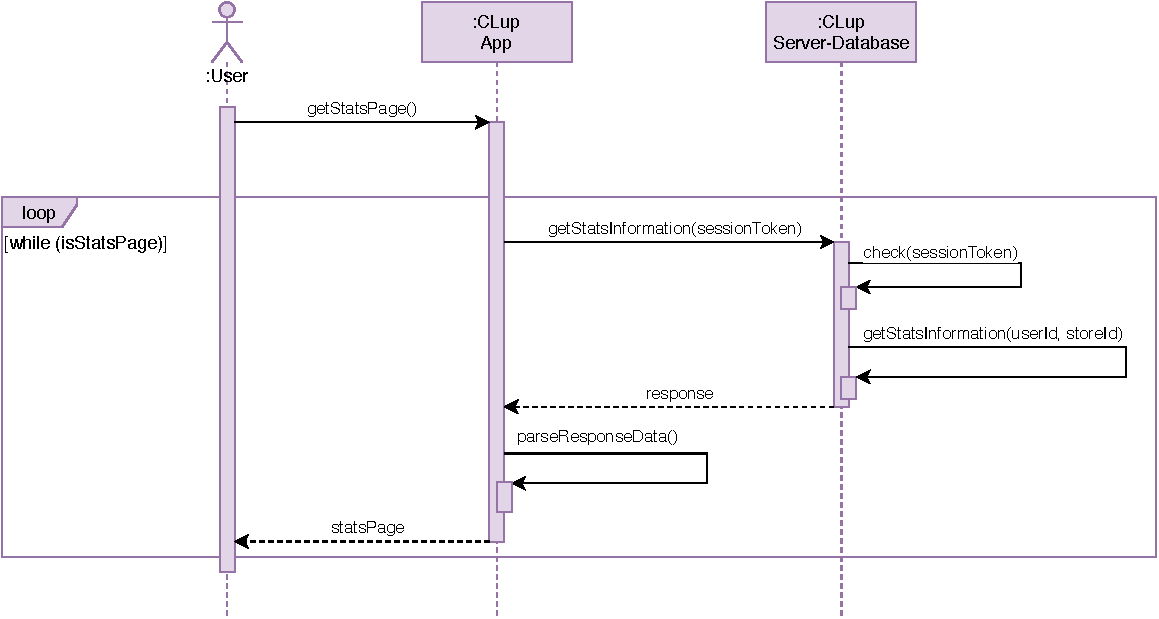
\includegraphics[width=1.0\textwidth]{images/getShowStatsPage_sequence_diagram.pdf}
	\caption{Show Stats sequence diagram.}
\end{figure}

\begin{figure}[H]
	\centering
	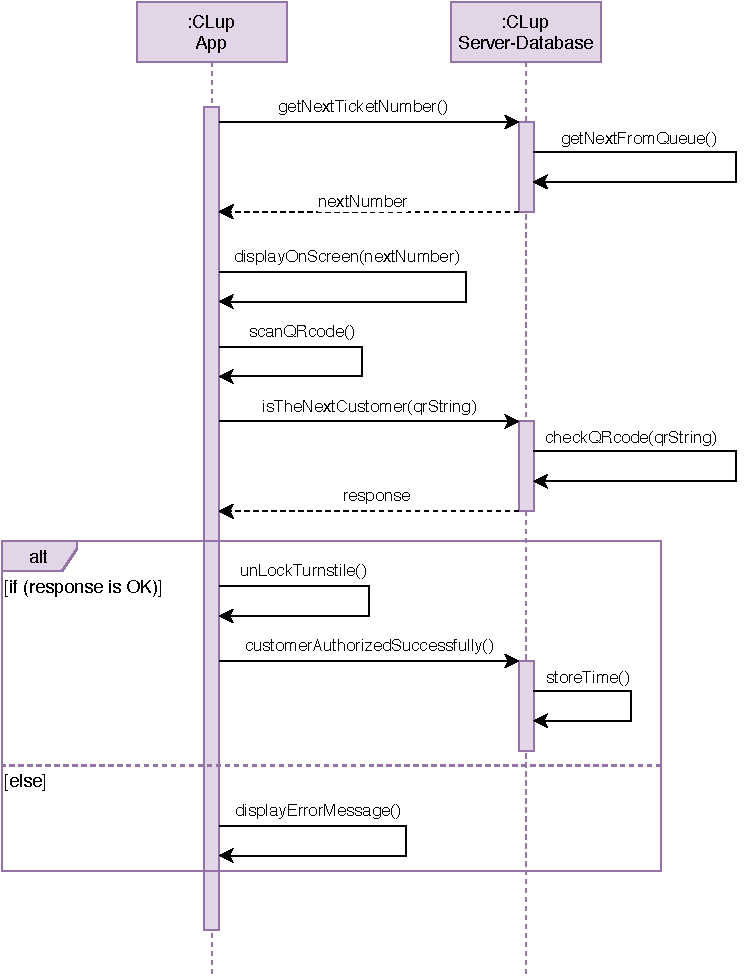
\includegraphics[width=1.0\textwidth]{images/authorizationToEnter_sequence_diagram.pdf}
	\caption{Sequence diagram reporting the activity periodically performed in background, by the application of the store manager, to authorize customers to enter in the store. For simplicity, the session authentication has been omitted.}
\end{figure}

\subsection{Mapping on Requirements}

\section{Performance Requirements}

We can differentiate our performance requirements in two categories:
\begin{itemize}
	\item The first ones are necessary to respect a goal, in our case are relative to the goal to limit the physical line situation in the proximity of the store. In 			order to achieve that, our application must precisely estimate the right time of arrival time of every single customer with an absolute error less than five 			minutes. That depends on the precise estimation of the position of the customer after lining up and a correct estimation on the duration of the customers time staying. Them also need to be under a certain value of error, for the first one the error must be less than ten meters instead the estimation of the time 	of the customer staying must be less than three minutes. Also, these estimations must not require more than twenty seconds to compute in order to be always relevant when it is shown to the customer.
	\item The second ones are required to guarantee a good level of \gls{qos}. Such as being able to manage at least a five hundred simultaneous user connections for each store, in order to let the all customer being able to line up, re-elaborate periodically the stats for the manager with a period less than one minute.

\end{itemize}
	

\section{Design Constraints}

\subsection{Standard Compliance}

All measurements are made by using the \gls{si} metric system: 
\begin{itemize}
	\item Distance [m]
	\item Time [s]
\end{itemize} 
All information regarding the users and the data collected by the application will be kept safe, more information in that regard will be stated on an agreement the user will have to accept. \gls{clup} pledge to respect what it will be written in that agreement. \\

\subsection{Hardware limitations}

The most important hardware requirements are the ones used by the store, necessaries for the basic function of the service. It must have two different hardware components:
\begin{itemize}
	\item One that has to acts as physical spot and so it is preferably a totem but in more general terms a tablet connected to a printer should suffice, and it is implied that the tablet or the totem should be also connected to Internet to communicate with the \gls{clup} server. The tablet is needed for letting people choose to get a paper ticket and the printer should print and hand it to them.

	\item The second component must be able to scan the QR code in order to let people enter when it is their turn and reject them when it is not their turn. So, it is preferably to have a turnstile with a scanner implemented on it for this purpose, it is also suggested to have a screen that shows the current position of the queue in order to reduce interactions.

\end{itemize}

There are also hardware requirements for the manager and the customers, the first one needs a device with a screen like a tablet, that is connected to Internet for the entirety opening hours of the store in order to let the manager control and manage the influx of people. The customers need a mobile device with Internet access and a \gls{gps} sensor, so a smartphone is preferred, in order to use both line-up and booking functionalities. 

\subsection{Any Other Constraint}

The user cannot line-up if he is already in line.
The user must give to the application permission to \gls{gps} during all the time he is in line, without this permission the user will be not able to look at his ticket and show the QR code.


\section{Software System Attributes}

\subsection{Reliability}
The \gls{clup} system should be operating continuously as much as possible, so it should be up for at least ninety nine percent of time. The faults and problem in the system should not occur during times where there is a high influx of people as they could cause the most dangerous situations. So, the system must contain some mechanism to increase its fault tolerance especially in critical periods of the day like peak hours of stores and have extra mechanisms during high load periods like holidays. An alternative of the required hardware of a store should always be available in case of failures, and they both should regularly checked. The collection of data is not a particularly important aspect of the application, but it should be still robust, so the data should be backed-up regularly in physical storage devices. 

\subsection{Availability}
As stated above, the operating time of the system, and so its availability, should be at least ninety nine percent of time. Scheduled maintenance should be programmed during the period between midnight and five a.m. since it is the period when most stores are closed, and the working ones have small load.

\subsection{Security}
The data collected by the application is not particularly sensible, but even so the applications should focus on keep it safe, by mainly encrypting the data before storing it and by using an encrypted channel to transmit it. Furthermore, the development of all components of the applications should be done in a way that considers the latest possible exploit and the possible vulnerability of the system and aiming to cover them all.  

\subsection{Maintainability}
The application should be designed by keeping in mind the design patterns of coding, such as dividing the application in functional components that are the least dependent on each other. So that their maintenance is done independently and does not spawn irregular behaviors and requires less downtime for the whole system to implement it. 

\subsection{Portability}
The applications should be available for Android and iOS operating systems. It should also be available for relatively older versions of these systems without it being a constrain and without reducing security standards.
